\documentclass[12pt,openright,final,twoside,extrafonts,ebook]{memoir}
\usepackage[utf8]{inputenc}
\usepackage[T1]{fontenc}
\usepackage[english,brazilian]{babel}
\usepackage[osf]{libertine}
\usepackage{leading,graphicx,epstopdf,hyperref,makeidx}
\makeindex

% Evitando órfãos e viúvas
\widowpenalty=10000
\clubpenalty=10000

% Escolhendo um estilo de capitulos:
\chapterstyle{bringhurst}
% Criando um modelo de páginas:
\makepagestyle{bringhurst}
	\makeevenfoot{bringhurst}{\thepage}{}{}
	\makeoddfoot{bringhurst}{}{}{\thepage}

\addtodef{\tableofcontents}{\clearpage\pagestyle{empty}}{}
\setlength{\cftbeforechapterskip}{2.3pt plus 2.3pt}
\renewcommand*{\insertchapterspace}{}


\checkandfixthelayout
% Começa o documento
\begin{document}

% Algumas definições puramente tipográficas
\pagestyle{bringhurst}
\parskip 3pt
\frenchspacing

% Começa a parte textual
\include{capa}
%título
\thispagestyle{empty}
\begin{center}
\vspace*{\fill}
\begin{flushright}
{\large\foreignlanguage{english}{It says little,\\
does less, \\
means \\
nothing} \\}

{\tiny (\emph{Do} Principia Discordia, \emph{página 00033})}
\end{flushright}
\end{center}
\cleardoublepage

%título, mais informações
\thispagestyle{empty}

\hrule

\begin{center}
{\scriptsize
Carol Peters\\
Duubhglas Juarezzz\\
Felipe Schneider\\
Peterson Espaçoporto\\
Rafael Beraldo\\
}
\vspace{.5cm}

{\Large Contos Discordianos}

\vspace{2cm}

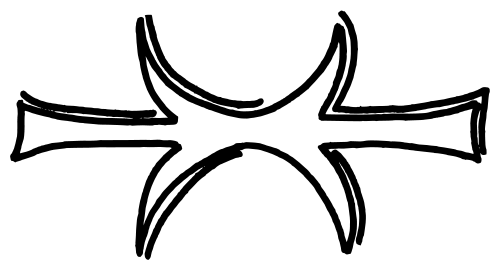
\includegraphics[scale=.35]{eris_hand}

\vfill

Avignon --- 3176
\vspace{.5em}
\hrule

\end{center}
\newpage

%página de burocracias
\thispagestyle{empty}
\begin{center}
{\tiny
CONTOS DISCORDIANOS

\vspace{.5cm}

\begin{minipage}[h]{.6\textwidth}
Alguns direitos reservados; esta publicação pode ser reproduzida e modificada de acordo com a licença \foreignlanguage{english}{Creative~Commons~3.0}. Veja suas liberdades e deveres em: \url{http://creativecommons.org/licenses/by-nc-sa/3.0/br/}
	\begin{center}
	
\includegraphics[scale=.2]{cc.eps}
	\end{center}
\end{minipage}

\vspace{.5cm}

\begin{minipage}[h]{.6\textwidth}
Edição por Rafael Beraldo \url{<revberaldo@cabaladada.org>}
\end{minipage}

\vfill

\begin{minipage}[h]{.6\textwidth}
Concluído e lançado na primavera de 3176 \textsc{yold} pela Imprensa Oficial da República de Avignon.
\end{minipage}
}
\end{center}

\newpage


\frontmatter

\newpage
\chapter{Introdução}

Schopenhauer uma vez disse: ``Ler significa pensar com a cabeça alhe\-ia em vez de pensar com a própria.'' Então permita-se pensar com a minha cabeça por alguns instantes. Visitar a história do discordianismo, como uma forma de entender por que nós estamos aqui e por que você vai se tornar mais um discordiano (aqui eu dou uma risada diabólica). Representante moderno de Carneades, o discordianismo é uma religião do ano de 1958\footnote{Ou 1959. (Nota do editor)} baseada no caos. Qualquer afirmação sobre o discordianismo nunca sobrevive a um exame mais minucioso. Isso porque divergir sobre o que são e o que fazem é lei entre os que se declaram praticantes do mesmo. Primeiro, porque para alguns o discordianismo é apenas uma sátira, uma piada disfarçada de religião. Para outros, na verdade é uma religião disfarçada de piada.
 
\begin{flushleft}
{\Large \textbf{Criação}}
\end{flushleft}

Os criadores do discordianismo foram Gregory Hill, também conhecido como Malaclypse the~Younger, que é o autor do principal livro, o \emph{Principia Discordia}, e Kerry Wendell Thornley, ou Omar Khay\-yam Ravenhurst, ou ainda Ho Chi Zen. Foi desenvolvido como um exercício de guerrilha ontológica no que eles chamavam de Operação:~Mindfuck através da ``versão Irmão Marx do zen'', o discordianismo.

\newpage
\begin{flushleft}
{\Large \textbf{Zen}}
\end{flushleft}

O discordianismo, embora a primeira vista não pareça, é o zen ocidental. Kerry Thornley, anos mais tarde de criar o discordianismo, sob o nome de Ho Chi Zen, lançou uma série de panfletos sobre a zenarquia. O zen nasceu na China, como uma escola do budismo mahayana, que é notável por sua ênfase na plena aceitação do momento presente, ação espontânea, e o abandono do pensamento julgamentoso e auto consciente. O zen ainda se divide em vários ramos, sendo mais notórios dois deles: Soto e Rinzai. Enquanto a escola Soto dá maior ênfase à meditação silenciosa, a escola Rinzai faz amplo uso dos koans.

Koans são histórias, diálogos, questões, ou afirmações geralmente contendo aspectos que são inacessíveis ao pensamento racional, ain\-da que possam ser acessados à intuição. Um dos mais famosos e que figura no \emph{Principia Discordia} é esse: ``Qual o som de palmas com uma mão só?'' Da mesma forma, o discordianismo faz amplo uso de histórias, diálogos, questões, afirmações, imagens e qualquer coisa que provoque a confusão, a Operação:~Mindfuck. O propósito é sacudir as pessoas de suas zonas de conforto e levá-las a pensar.

\begin{flushleft}
{\Large \textbf{Caos}}
\end{flushleft}

Os discordianos que seguem o erisianismo usam Éris, a deusa grega da discórdia, como divindade. A palavra caos irá aparecer muitas vezes no material discordiano. Sobre tal é dig\-no de nota que, para um discordiano, caos não é antônimo de ordem. Para eles, o caos é a natureza da realidade. O antônimo de ordem é a desordem. Eles apenas querem conscientizar a sociedade moderna, que busca a ordem em tudo, de que vivemos em um Universo caótico e que não existe essa coisa que chamamos ``verdade''. Como escreveu Robert Anton Wilson, também conhecido como Dr.~Mordecai Malignatius, no meio discordiano:

	\begin{quote}
	{\small
	A iluminação discordiana é alcançada quando você se conscientiza de que, apesar de a deusa Éris e de a Lei dos Cinco não serem literalmente verdadeiras, nada é literalmente verdadeiro. Dos cem milhões de sinais zunindo, recebidos a cada minuto, o cérebro humano ignora a maioria e organiza o resto em conformidade com qualquer sistema de crença estabelecido nele. Podemos selecionar sinais ordeiros e legais e dizer que tudo é projetado por uma inteligência cósmica, como no tomismo, ou selecionar sinais caóticos e afirmar que Deus é uma Mulher Louca, como no discordianismo. O cérebro ajustará os sinais recebidos aos dois sistemas de crença\ldots\,Ou a uma dúzia de outros.}
	\end{quote}
 
\begin{flushleft}
{\Large \textbf{Brasil}}
\end{flushleft}

Não é certo quando o discordianismo chegou ao Brasil. Mas foi graças à sua presença na Internet que ele conseguiu continuar existindo em nossas terras. Nos últimos anos, com o avanço de algumas descobertas em psicologia e física se aproximando dos ideais pregados pelo discordianismo e o crescimento de sua presença na Internet, ocorreu um aumento no número de seguidores.  Mantinha-se comunidades em redes sociais com gatos pingados aqui e ali discutindo a filosofia enquanto digitavam ``fnord'' aqui e ali ou discutiam se o gato de Schrödinger estava vivo ou morto. Então, foi traduzido o \emph{Principia Discordia} em português por um sujeito franzino, egoísta, megalomaníaco e que gosta de falar de si mesmo na terceira pessoa. Atropelado por uma moto enquanto ia para seu trabalho de bicicleta, ganhou um afastamento médico de quinze dias. Sem nada para fazer a não ser ler, resolveu traduzir o livro que considerava o ápice da espécie humana. Pegou um caderno com a capa do Bob Esponja e se lançou à tarefa da tradução.

Pouco tempo depois ele iniciou um blog que se declarava uma Cabala Discordiana. A Cabala 1001~Gatos de Schrödinger atraiu religiosos raivosos, adolescentes na puberdade, artistas, políticos, pedófilos, pessoas grosseiras e um pequeno grupos de pessoas que mais tarde, sem embaraço nenhum, iriam se declarar discordianos. Iniciou-se um pequeno movimento que gerou a criação de cabalas e a criação de uma rede social entre os mesmos.

Os contos aqui reunidos são de pessoas que de alguma forma tomaram contato com o \emph{Principia Discordia} e que de uma forma ou outra sentaram suas bundas em suas cadeiras e escreveram coisas fodásticamente incríveis ou ridículas, deixo o juízo estético para cada um de vocês, em especial Kant. Não é interessante como essa coisa funciona? Num dia um idiota qualquer é atropelado, coloca-se a traduzir um livro escrito por um bando de loucos americanos que não tinham qualquer objetivo a não ser tirar um sarro de todo o Universo e faz com que um bando de garotos selvagens e avatares de Éris escrevam coisas mais ou menos relacionadas com tudo aquilo. Do pouco que eu conheço do idiota em questão, acredito que ele esteja orgulhoso.

Felipe Schneider, o sujeito que abre este livro, me pegou de jeito, o sacana. Prende a leitura. Carol Peters é puro ouro. Ou melhor, uma maçã de ouro puro. Sobre o Rev.~Rafael Beraldo eu não posso dizer nada, pois como ele é quem é o diagramador, tenho medo do que o bastardo possa fazer, colocar palavras na minha boca só para me difamar, por exemplo. O Duubhglas Juarezzz é tipo a nossa Hebe Camargo, discordiano \foreignlanguage{english}{\emph{old school}}. E escreve incrivelmente. Já o Rev.~Peterson é o nosso Kaká. Jovem e craque. Aliás, já que nosso país tem uma relação com o futebol muito forte e as metáforas relacionadas ao mesmo sempre vem a calhar, com este time nós ganharíamos a Copa. Diversas vezes. Pentacampeão, com certeza.

Logo, a história do discordianismo no Brasil passa por aqui. Por estas palavras. E vai continuar nas palavras dos contos a seguir. E continuará, quem sabe, nas suas ações e palavras. Sim, estou falando com você. Se você nunca se imaginou sendo discordiano um dia, é tarde demais. Nós já pegamos você.

Qual o parasita mais resiliente? Um vírus? Uma bactéria? Um verme intestinal? Não. Uma ideia. Uma ideia pode reescrever todas as regras e mudar o mundo. E a ideia do discordianismo continua por aí, pegando algumas mentes-que-realmente-pensam desprevenidas e as convertendo instantaneamente. O discordianismo não faz prisioneiros. Mas definir o que ele é? Esqueça. Seja ele uma piada disfarçada de religião ou uma religião disfarçada de piada, parece que o discordianismo veio para ficar.

	\begin{flushright}
	\emph{Ibrahim Cesar},\\
	Primavera de 3176 \textsc{yold}
	\end{flushright}

%\begin{flushleft}
%{\Large \textbf{Referências}}
%\end{flushleft}
%
%{\small
%\noindent\textsc{mal}-2. \emph{Principia discordia}. Tradução brasileira: Ibrahim Cesar, 2005\\
%\noindent\textsc{wilson}, Robert Anton. \emph{A Nova inquisição}. Madras, 2004\\
%\noindent\textsc{wilson}, Robert Anton. \emph{O Gatilho cósmico}. Madras, 2004\\
%\noindent\textsc{wilson}, Robert Anton. \emph{The Illuminatus! trilogy}. \foreignlanguage{english}{Dell Publishing}, 1984\\
%\noindent\textsc{alhazred}, Abdul. \emph{Necronomicon}. Tradução para o latim: Ola\-us Wormius, 1228\\
%}


\tableofcontents

\mainmatter

\thispagestyle{cleared}\part{Felipe Schneider}
\chapter{Sobre Macacos e Bananas}

Acordo. Olho o relógio. São 8:23 da manhã. Só mais cinco minutos. Acordo. Olho o relógio. São 8:28. Me levanto. Como algumas bananas acompanhadas com Co\-ca-co\-la Ze\-ro.

Estou seguindo essa dieta rigorosamente desde o início da semana, na tentativa de manter mais triptofano no meu cérebro durante o dia. Segundo Aldous Huxley, nossa mente só consegue receber uma certa quantidade de informação diária, devido a fatores evolutivos, desenvolvidos na época em que éramos mais macacos que homens. E um bom jeito de ``ver mais do que o normal'' seria através de drogas alucinógenas. Robert Anton Wilson recomenda a maconha, embora não seja por muitos considerada alucinógena, porém reconhece o maior poder de outras, como o \textsc{dmt}, a salvinorina, o \textsc{lsd}, a serotonina e o \textsc{lsa}.

\begin{sloppypar}
Como eu não quero ``ver mais que o normal'' atrás de uma jaula, ver o sol nascer quadrado, finjo ser um macaco a comer bananas, que contém triptofano, precursor biológico da serotonina. Engraçado, este é um arquétipo símio bastante pobre, semelhante ao que temos dos coelhos, de que comem só cenouras. Se fosse eu um macaco, além de quase não comer bananas, já estaria certamente atrás de uma jaula. Não parecem funcionar, tanto as bananas, quanto as jaulas, para qualquer fim que seja.
\end{sloppypar}

Mas, sinceramente, não sei bem para que serve a Co\-ca-Co\-la Ze\-ro.

Depois de um banho, já estou pronto. Corro para pegar o ônibus. No ponto, olho o relógio. São 9:23 ainda. Espero cinco minutos e pego o primeiro \textsc{ufsc} semi-direto que encontro. Um carro da Transol, de número 0235. Não sei para onde vão essas latas azuis no final do dia mas, com certeza, vão todas para o mesmo lugar. Devem ser muitas e, como são todas iguais, não só é inteligente como indiscutivelmente necessário numerá-las. No fim, o ``0235'' serve justamente para pôr ordem naquele maldito lugar, seja lá onde for. Ônibus nessa cidade nunca foram rápidos, ainda mais que o meu destino é o terminal viário do centro.

Chego. Olho o relógio. São agora 9:55. Demorei, pensei. Vou ao chafariz do terminal. Aqui, no terminal municipal, existe um belo chafariz, como que para entreter os passantes com a água que, além de não a beberem nem a usarem para refrescarem-se --- certos estão eles, claro, afinal, não são animais, que nojeira seria! --- só a veem cair, cair e cair. Tentem fazer um chafariz em que a água só sobe, sobe e sobe. Ai então vão \emph{realmente} entreter os passantes.

Me sento em um banquinho, sorte de haver encontrado um. Um desses quadrados. Digo, cúbicos. Na verdade, cha\-mam-no de ``banquinho'' por consideração, carinho. É um bloco de concreto que, ao brotar do chão, revestiram com cerâmica, dessas bem baratas. Mas ainda assim serve muito bem para sentar.

Espero. Olho o relógio. 10:05 ainda. Logo chega uma garota, não muito alta, não muito baixa. De um ruivo que confunde. Será que é castanho? Não, na luz parece mais um loiro escuro. Estranho. Veste um, lógico, vestido. Fantástico. De cor indistinguível para mim, já que sou daltônico. Daltonismo é algo engraçado. Todos pensam que faz a pessoa ver em preto e branco, enquanto que na verdade apenas confundimos alguns tons, trocamos algumas cores. No meu caso, por exemplo, confundo alguns violetas por azul, alguns amarelos escuros por verdes e uns tantos azuis claros por tons de cinza. Com certeza ela observa cores melhores que eu. É que o daltonismo está relacionado com um gene recessivo no cromossomo masculino. Quer dizer que mulheres passam a desordem aos seus filhos, mas só a manifestam os homens. Discreto, sinceramente humilde o vestido, como de uma dama oriental. Mas ainda assim, digo, fantástico. Ouso dizer, digno de uma divindade seria. No específico caso, o é.

--- Vago está? --- pergunta a garota, agora sem poder ter a idade reconhecida. Que absurdo, seriam dezenove anos? Seriam trinta?

--- Claro, desde que não me arranque o sol --- respondi.

Sentou-se no ``banco'' atrás de mim. ``Atrás'' é discutível. Estes assentos são perfeitamente simétricos, senta-se na posição que agradar. No momento, estava eu sentado de costas para o sol, abraçando minhas pernas de leve. Ela então senta-se no banco ao lado, mas de frente para minhas ensolaradas costas.

--- O sol parado está, nem eu posso de lá o tirar.

--- Falo sobre as ondas eletromagnéticas que emana, não quero que teu corpo produza obstáculo para as pobrezinhas até meu corpo. Absurdo seria se com isso o sol se deslocasse. Haveria motivo para que pudesses fazê-lo?

--- Claro que sim. Digo, claro que não.

--- Entendo. --- Na verdade, porra nenhuma.

--- Somente digo. Remédios psiquiátricos, os tomo. Tente evitá-los. Não vão te bem fazer.

--- Quê? --- Me viro para olhá-la melhor, de espanto. Seria o português sua língua nativa? Pois não parece\ldots

--- Com essa tua dieta, haverias de várias dores de cabeça horríveis ter.

--- Dieta? --- Grandes olhos ela tem. Azuis ou cinzas? Talvez um verde muito claro. São como dois caleidoscópios.

--- Bananas. Queijo nesses tratamentos também deves evitar. Se não queres enxaquecas ter.

--- Mas eu não estou em nenhum tratamento desse tipo\ldots\linebreak E como sabes das bananas?

--- Não o sei. É tu quem sabes.

--- Quem és tu?

\begin{sloppypar}
--- Com certeza psiquiatra não sou. Sobre a guerra de Troia, já leste?
\end{sloppypar}

Onde está?

Acordo. Olho o relógio. São 8:23 da manhã. Só mais cinco minutos. Acordo. Olho o relógio. São 8:28. Me levanto. Como algumas bananas acompanhadas com Coca-Cola Zero\ldots

\chapter{Ode ao `quase'}

Uma pequena perturbação nas folhagens, um gemido do vento, um assovio das árvores. Quatro horas da manhã. Tarde assim da noite, os pássaros começam, timidamente, a cantar, como num murmúrio que se expande pelo profundo teatro, revelando então um coro \emph{a cappella} ao final.

Enquanto o tempo passa, ainda antes de o sol nascer, aque\-le astro que, ao aquecer as folhas faz vibrar o mundo e entra em gozo com os arbustos, como num clímax de homem e mulher, de céu e terra, os pássaros entram em frenesi. Algo está para acontecer, o grande segredo de tudo, este está para ser revelado. Está para ser relevado.

Se há um mistério digno de se revelar, excitante de se esconder, há um mistério que, ao se contar, tem-se o desejo saciado, como num depoimento, quando a testemunha, suando e aliviada, pode voltar para o calor do lar, do sol, ao ouvir, daquele que tem o torso adornado com as letras `s', `g' e `t', as palavras ``pode ir''. Vai. É o momento primordial. Se é mais noite a medida que o dia se aproxima, assim como se é mais humano a medida que o momento derradeiro chega. Se acaba, se é mortal. Se é.

O segredo é mais segredo segundos antes de ser contado, intervalo de tempo lembrado por quem o ouve e diz a si mesmo que agora o sabe, mas há pouco não sabia. Quando se é segredo no auge, tem-se que definhar, morrer, deixar-se contar, deixar de se esconder, deixar de ser segredo.

Os raios já vão aparecendo. O regozijo dos pássaros, que há instantes era colossal, agora mais parecem os gemidos de prazer em brasas, como de uma fogueira que quase se apaga: breve, profunda, mas ainda quente. Ah, como é linda a noite!

Já se é dia novamente.


\part{Carol Peters}
\chapter{Ao Teu com o Diabo}


\begin{center}
{\Large \textbf{I}}
\end{center}

``Não existe ateu em avião em queda''. É o que não cansam de repetir os crentes e eu, em meu agnosticismo de ateu, nunca dei crédito à premissa.

Eis que, rumo a Madrid para um simpósio, meu avião entra em turbulência.

Não pense você que, por não acreditar em Deus, tenha na ciência o depósito de minha fé. Em parte sim, é verdade. De todo modo, não vejo muita distinção entre os fanáticos religiosos e alguns cientistas, em especial os físicos, que nunca vi povinho mais dado a acreditar em teorias completamente lunáticas.

Posto isso, não é exagero dizer que tenho medo de voar, até porque o que sinto é, senão, verdadeiro pavor! Tremi todo junto com a aeronave e recostei-me na poltrona com os olhos fechados. Logo que a situação se regularizou, as comissárias correram aos seus carrinhos para servir os lanches, antes que não fosse mais possível.

Conhecendo meu sistema digestório sensível e já prevendo uma próxima instabilidade, dispensei meu lanche, servindo-me apenas de um pouco de álcool. Recostei-me novamente, de olhos bem abertos dessa vez, e comecei a distrair-me com pensamentos aleatórios.

Acabei entrando na questão de meu ateísmo; se não era o caso de eu ser agnóstico, talvez\ldots\,Estava a ponto de puxar conversa com o agnóstico sentado ao meu lado --- já o conhecia de uma outra conferência qualquer, mas por não saber seu nome e não querer interromper a degustação que fazia de sua xícara de chá, vacilei, analisando a melhor forma de abordá-lo --- quando entramos em uma nova turbulência.

Mais uma vez me subiu um frio na espinha e, não tendo o avião se reestabilizado relativamente rápido --- como ocorreu na anterior --- o pânico começou a se instaurar no interior da cabine. Ao tentar desviar meu olhar do desespero alheio, acabei por mirar a janelinha e a tempestade que se dava lá fora. Baixei com violência a persiana, olhando para o teto e exclamando um ``ai meu Deus!'', vício de linguagem que eu havia há muito apagado do meu vocabulário.

Passado o choque de meu apelo inconsciente, o pensamento nefasto de que apenas uma força espiritual me salvaria tomou conta de mim. Nesse momento percebi a diferença nada sutil entre o agnóstico e o ateu (imagine que, em meio àquele caos, meu colega continuava concentrado em seu chá, como se nada estivesse acontecendo ao seu redor).

Assim que admiti para mim mesmo que minha única salvação seria divina, comecei a pensar em para quem rezar. Não poderia abrir mão de comer carne, tampouco colaborar com alguém que manda seus fiéis apedrejar mulheres. Minha mãe não era judia e o panteão latino era taylorista por demais, nunca saberia para quem apelar nessa circunstância.

Restou-me o deus cristão, mas tinha lá minhas dúvidas de que Ele era de fato ``só amor''. Durante minha vida, nunca fui lá muito simpático com Sua omnissapiência e não O imaginava muito inclinado a perdoar minhas bastantes heresias a tempo de salvar-me do acidente iminente.

Num flash de razão, lembrei que admitir a existência de um Deus era aceitar igualmente sua antítese. Depois de uma breve entrevista com minha consciência, decidi vender minha alma imortal ao Diabo, ao preço da salvação de minha vida terrena.

Dos males, o menor. Sei lá se por isso ou não, a voz do piloto logo soou, avisando que já havíamos voltado ao normal e pousaríamos em Madrid dentro de vinte minutos.

\begin{center}
{\Large \textbf{II}}
\end{center}

Engraçado que sempre considerei os agnósticos ``ateus fracos'' e acreditei piamente que o ceticismo radical fosse muito mais ``seguro'', devido seu caráter estável-estático.

Quem sabe seja exatamente nessa estabilidade, na solidez ideológica, que esteja o ``perigo''. Confesso não ser o maior entendedor das questões físicas, mas não é verdade que as edificações precisam de um certo balanço pra que não sejam derrubadas pelo vento ou tremores de terra? Por que seria tão diferente conosco, humanos, a ponto de considerarmos os flexíveis fracos e jogarmo-los no balaio dos indecisos e irrelevantes?

Sei que nesse meio tempo, em que me entretinha com tais questões, minha mala deu algumas voltas na esteira (vi de relance um volume amarelo passando e descarto a possibilidade de outra pessoa no mesmo voo ter uma mala de viagem amarela).

Não digo que me conformei, apenas que mais uma vez as futilidades do mundo externo acabaram suprimindo minha abstração.

Retirei por fim a tal mala amarela da esteira e rumei para o saguão. Um rapaz qualquer segurava preguiçosamente uma plaquinha precária, improvisada de um pedaço de papelão em que meu nome fora escrito com caligrafia primária, um ``T'' a menos, um ``C'' a mais e alguns respingos de gordura que eu não cheguei a ver, mas pude perfeitamente imaginar.

Bem, não havia muito que pudesse ser feito. Cheguei-me a ele, impaciente para ser levado de uma vez ao hotel, torcendo para que fosse daqueles condutores silenciosos e rápidos. Nenhum-nem outro; desatou a falar comigo.

Primeiramente, disse que não sabia quem eu era. Óbvio que não; não sou o tipo de pesquisador que recorre à mídia de massas. Tenho alguma dignidade --- arrogância academicista, como queira. Então\ldots

``Comecei a pesquisar. Não é todo dia que\ldots\,Na verdade é mais comum do que você deve imaginar, mas enfim. Tinha que saber alguma coisa sobre quem eu estava levando. E devo dizer que foi um ótimo negócio. Um pesquisador tão importante quanto você\ldots\,O que paguei por sua alma foi uma niñeria!''

Talvez porque nesse momento um carro nos fechou no cruzamen\-to e começaram a soar buzinas de todos os lados, acabei alucinando as últimas sentenças dele. Fiquei meio assim de pedir que repetisse, pareceu um pouco deseducado de minha parte. Mi culpa; não prestava mesmo muita atenção já que o assunto dele não me era interessante.

Só para não dizer que pouco me importava, assim que deixamos o furdúncio do cruzamento tomei os cuidados de perguntar seu nome.

	\begin{center}
	\emph{Os movimentos finais de ``Ao Teu com o Diabo'' ainda dormem desconhecidos no caderno da jovem Carol~Peters.}
	\end{center}


\part{rev.~Rafael Beraldo}
\chapter{Amor, Sublime Amor\ldots}

Arthur entrou no costumeiro bar, sentou-se no lugar costumeiro do balcão; estava ansioso pelo jogo. Esperava fervorosamente que a Colômbia desbancasse o Brasil --- mas é claro que não diria isso para o povo ali, ou seria enxotado.

--- 'Noite, Hetz. Feliz dia do Nietzsche.

--- Boa noite, professor. Feliz dia do Bigode! --- E Hetzlinger riu bastante. --- E, ah, claro, feliz dia dos professores também. Veio assistir ao jogo, é?

--- Podes crer. Nem me lembre que fui professor, argh. Me vê o de sempre.

O bartender começou a preparar a bebida do velho Arthur, e, enquanto este esperava pelo jogo, João chegou, batendo-lhe nas costas e desejando feliz dia do Bigode. Enquanto isso, o Jornal Nacional rolava solto na TV do bar e uma notícia chamou a atenção de João:

--- Hoje, por volta das nove horas da noite, acabou o drama de Heloá, a jovem de 15 anos que estava sendo mantida como refém de seu ex namorado, Lindembergue Fernandes Alves, de 22 anos, inconformado com o fim do namoro\ldots --- o bartender abaixou o som da TV e comentou para Arthur e João:

--- Horrível isso aí, não? Um cara desses merecia\ldots

--- Merecia nada, cara. --- Arthur interrompeu Hetz, causando espanto neste e em João. --- É mais que natural que esse tipo de coisa aconteça. E, depois, não é ele que está fazendo isso, mas o gênio da espécie.

--- Xiiii, tu vais começar a viajar de novo, é, professor Schopenhauer? --- o bartender falou, e voltou a limpar copos, deixando o volume da TV alto novamente. João, porém, após pensar um pouco, acabou por concordar com Arthur.

--- Hetz, Arthur tá certo. Lembro de um trecho de \emph{EQM} que fala sobre isso.

--- \emph{EQM}? --- Arthur perguntou.

--- É, o livro do papa Ibrahim Cesar. Literatura discordiana. Nunca leu?

--- Não, eu parei de ler.

--- Parou de ler, mas e a bebida? --- o velho filósofo fez um sinal de reprovação. --- De qualquer forma, eu me lembro bem do que o livro fala. É Falls, a namorada do protagonista, quem fala sobre a comunicação e como isto pode revelar como nos relacionamos com as pessoas. Olha só o que diz Falls:

\begin{quotation}
Voltando ao que eu queria dizer, esse pensador, Martin Buber falava de dois modos de expressão entre as pessoas. Ele falava da comunicação, entende? A comunicação se expressa de duas formas. EU-TU e EU-ISSO. O EU-ISSO é usado em nossas relações com o mundo das coisas. Essa é a minha casa. EU-ISSO, entende? O EU-TU são nossas relações com seres humanos. Eu quero passar o resto de minha vida com você. EU-TU.
\end{quotation}

--- Certo. Então você quer dizer que a relação entre Lindembergue e Heloá chegou à esta condição de eu-isso? --- Schopenhauer começou a pensar sobre isso. --- Realmente, faz sentido, mas, como eu disse ali em cima, isso tudo foi causado pelo gênio da espécie. Explico: o amor não existe; o que existe é a vontade da vida se perpetuar noutro ser, num terceiro ser, e isso é o que faz surgir a admiração por alguém. Explicar tooodo o mecanismo seria um tanto enfadonho agora, portanto, fico por aqui, só para apresentar minha conclusão: Lindembergue não merece nenhum tipo de punição, apesar dos pais deles merecerem pelo péssimo gosto ao escolher o nome do filho; ele está sendo movido por algo que é maior que ele, maior que todos os desejos dele. Afinal, o que pintam todos os poetas e depois chamam de amor é, tão somente, algo que é transcendente a eles e, portanto, não podem entender em sua plenitude. Porém, o amor acaba quando ele realiza seu desejo: criar um terceiro indivíduo.

--- Schop, te digo mais: Nietzsche concordaria contigo quanto a isso de não punir o cara --- exclamou Hetz --- já que o Bigode disse, em \emph{Assim Falou Zaratustra}:

\begin{quotation}
\noindent Sempre se viu só, como o autor de um\\
ato. Eu considero isso loucura; a\\
exceção converteu-se para ele em\\
regra.\\
\end{quotation}

Então, os três se olharam, olhavam para a TV, e Schopenhauer disse:

--- Muito bom, gente, mas, agora, eu tô afim é de assistir o jogo. Tá pra começar.

\chapter{Retirado de um velho pedaço de jornal}

{\Large \textsc{mais que autoajuda, escritor promove o autoconhecimento}}

São Paulo --- Ontem (23) ocorreu o lançamento do livro \emph{O hippie que não era sujo}, de Astolfo Voltaire, pseudônimo de Alberto J. Goldsmith-Paes, o internacionalmente famoso multimilionário brasileiro. O livro, custeado por ele mesmo e editado pela ed. 3K, foi lançado ``chiquemente'' no distinto hotel de São Paulo, com banda contratada e distribuição de exemplares entre os presentes.

A equipe deste Jornal conseguiu uma descontraída entrevista de vinte minutos com Goldsmith-Paes.

\emph{Pergunta --- Como foi que você resolveu lançar o livro} O hippie que não era sujo\emph{? Comente um pouco sobre seu conteúdo.}

\textbf{Goldsmith-Paes ---} Resolvi lançar o livro quando notei que existia um conflito muito gran\-de nas pessoas, principalmente entre os jovens, entre ganhar dinheiro ou carregar nobres ideais como amor, sinceridade, compaixão, empatia, altruísmo. Muita gente vinha e me perguntava, ``Alberto, mas como você consegue conciliar essas coisas? E a exploração etc.?'' Eu realmente não tinha parado para pensar nessas questões até então. Mas pensei e achei algumas soluções. Quanto ao conteúdo, ele se relaciona diretamente com o título: um \emph{hippie} em plenos anos sessenta que deseja seguir os passos do pai e se tornar bem-sucedido, mas ao mesmo tempo se identifica com os ideais de seu tempo.

\emph{P --- E a escolha dessa personagem foi feita por qual motivo?}

\textbf{G-P ---} Creio que esses belíssimos sentimentos de que trato no livro são rapidamente relacionados ao movimento \emph{hippie}. É o acontecimento do tipo mais conhecido e temporalmente perto de nós. Esse foi o motivo pelo qual escolhi um \emph{hippie de coração}: ele vivia num momento de tensão máxima, então representa bem o conflito pelo qual passam algumas pessoas.

\emph{P --- Algumas pessoas classificaram seu livro como de \emph{auto\-ajuda}. Isso te incomoda? Como você o classificaria?}

\textbf{G-P ---} A última pergunta primeiro. Eu prefiro não clas\-si\-ficá-lo. Acredito que seja do tipo de coisa nova, mas sempre há quem acabe por classificar. Por outro lado, chamá-lo de \emph{autoajuda} não é completamente ruim, só não capta tudo o que o livro traz. Ele é muito mais que autoajuda, já que toda a ajuda que a pessoa precisa está nela e não no livro. \emph{O hippie que não era sujo} apenas guia as pessoas por esse caminho que é a mente delas, suas ideias.

\emph{P --- O público esperado é majoritariamente jovem?}

\textbf{G-P ---} Sim. Mas é um livro para todos, e não só aqueles que desejam ser financeiramente bem-sucedidos. Ele tenta conciliar as contradições do mundo em que vivemos e, eu acredito, é muito eficiente em atar as pontas. O livro é uma realização, de todo modo.

Alberto Godsmith-Paes é também conhecido por escrever o ``livro-cartilha'' \emph{Cinco maneiras para não reagir a um assalto}, onde alterna o tema explícito no título com bom humor, contando experiências suas e de conhecidos, e também o livro \emph{O que os golfinhos não podem fazer}, onde faz uma análise otimista das conquistas e rumos da humanidade.

\chapter[Nos Bastidores da \textsc{tv} e da Religião]{Enquanto Isso, nos Bastidores da \textsc{tv} \& da Religião\ldots}

Brasília. Oásis de brilho parco, concrético. Las Vegas brasileira.

Bancas de jornais ardiam às três da tarde. O sol evaporava violentamente o espelho d'água. Faxinavam um corredor de Nova Versalhes. Carros jorravam $\textrm{CO}_{2}$ no deserto. Um fardado de terno olhava a cidade pela persiana da janela ministerial. O celular tocou. Tirou-o do bolso, abriu, deixou que a sombra cobrisse seus olhos, e atendeu. Alô?

``Ah, consegui te ligar. Estou indo praí, e o sinal estava péssimo. Deixe-me explicar o que está acontecendo, posso?''

``Vá em frente.''

``Ótimo. São muitas coisas. Menciono algumas: o \textsc{ibope} da Record. Você sabe, eles nos ultrapassaram. Isso não parecia ser um grande sinal, na realidade\ldots\,E algumas pessoas daqui me disseram que talvez fosse melhor se manter na retaguarda e não correr riscos ainda. Mas quem manda pensa diferente. Além disso, há um projeto de lei aí. Noticiaram isso hoje, eu digo, mas ninguém sabe muito bem o que pode virar. É algo sobre mais poderes religiosos, não sei bem. É um dos motivos pelo qual estou indo aí. Por outro lado, tem esse acordo com o Vaticano\ldots''

``Vocês não estão indo longe demais?''

``Não, quero dizer, o Vaticano não vai nos comprar. Não estou sugerindo nada sobre o Vaticano. Mas o número de crentes está enorme, você sabe. Esse Edir Macedo tem todos esses rolos que estamos soltando, mas isso precisa de uma ajuda de vocês também. Nós estamos tentando libertar a população do feitiço\ldots\,Olhe, há quem se vicie em pagar o dízimo. Então viciam no canal da igreja. Estou indo direto demais ao ponto?''

``Estou acostumado.''

``Ah, sim. Bom, eu nunca fiz isso, mas me pediram pra ser sincero. Ou inventar alguma sinceridade que pareça ser de utilidade pública. Bom, vocês são a utilidade pública, e nós temos o poder pra divulgar\ldots\,Ainda. Quero deixar claro: não é algum tipo de lobby. Mas isso simplesmente não pode chegar a um nível que vire uma jihad --- e você sabe que há quem goste da jihad aqui.''

O fardado suspirou. ``Eu sei.''

``Perfeito. Há uma janta marcada. Estou te convidando. Vo\-cê pode ir?''

``\ldots\,não sei. Podemos conversar quando você chegar?''

``Sim, claro, mas pense que essa janta pode ser útil pra vocês e para nós, e podemos torná-la boa para você e para mim.''

O fardado parou pra pensar. O cara que liga é meio novo. Mas ele vem com instruções do que falar, e isso não é pouco. Disseram para esperar pela ligação, e quem disse não é gente de se ignorar. Tencionar um pouco pro lado do garoto não fará mal.

``Vamos deixar isso meio certo. Preciso verificar agenda e essas coisas. Falamos quando chegar.''

``Me disseram que vão me largar na frente do museu, na Praça dos Três Poderes. Dê uma passada ali, eu te ligo quando estiver lá. Tente não trazer mais gente, não estou acostumado com isso.''

``Perfeito. Bom resto de viagem. Até mais, abraços.''

O cara que ligou se despediu.

Aquilo era sério.

\chapter[Um conto em três actóides]{Um conto em três actóides (que também serve como exercício proppiano da faculdade)}

Ato um: era uma vez. Muito feliz. Ela pediu: vá, minha filha, Joana. Mas\ldots\,Me promete? Prometo, mãe. E foi. Como muito jovem, ignorou o mas anterior. E continuou indo. Então parou. Um môço. Antônio E., nome dele (lobo, esse lobo do homem). Família nobre, Moraes. Sem morais. Sem mais: diálogo: ?, ., ?, ., ?, \ldots\,Sim, caminho melhor, esse, Joana. E Antônio E. foi. Joana logo também. Voltas, voltas, voltas, demorou, chegou. Entrou, aberta. Gritos. Vó?

\begin{center}
\emph{(Fecha o cenário mental, abre outro. Terras longínquas, aparece Siegfried. De escopeta, não espada.)}
\end{center}

Ato dous: com cabeça de dragão inda rolando, passa Siegfried, herói da gente deles, e ouve gritos. Qué que houve? Ele só ouve. E se'proxima. Por Jesuis Shiva Thor!, comeu a vó e a criança, maldito seja! E tenta se aproximar, nosso herói, mas encontra os seguranças. Bang, bang, BANG, isto é, tiros. Carnificina. Lobo Antônio foge. Helicóptero. Aparece a Valkyrja, die walküre, e cena de perseguição. Narrador: ``eis que na avenida perseguição inusitada, três carros de polícia atrás de cavalo e helicóptero''. Mundo lóki. 'Caba a gasolina (especial, evidentemente) do aeromóvel a garota do cavalo sorri pára Siegfried o herói saca'escopeta e mete três tiros nos cornos do lobo ufa.

\begin{center}
\emph{(Por sorte, Joana e sua avó saem vivas da barriga do homem de taras estranhas que as comeu. Metabolismo lento, saravá.)}
\end{center}

Ato three: eis que'á Justiça chega, heroína da nossa gente. Salvadora, de papel timbrado, a enxugar o sangue derramado. Fala-se, não se mata um homem assim, não. Por mais bizarras as taras. Não: sociedade, julgamento certo ele merecia. Sem pedras \& paus, com papéis e fala, Siegfried é perseguido, porcos atrás dele. Dá uns tiros, monta no cavalo da Valkyrja, dispara com vovó e Joana atrás. Deixa vovó em casa, com cesto de doces e curadíssima. Voltando pra casa de Joana. Mamãe é muito sozinha, e mostra uma foto. Herói solitário, se interessa. Mas a Justiça os pega. Siegfried em cana, Joana em casa, felicidade geral, sai no jornal. Julgamento: demora. Siegfried espera, argumenta, acha bom advogado. ``Era um demônio, aquele lobómem''. Júri divido, no fim concorda (martelinho batendo; veredicto). ``Um demônio'', agora a opinião pública convencida recita. Vilão morto, dinheiro doado prálguém. Siegfried casado, com a mãe. Joana claustrofóbica pra sempre; ``vai virar lésbica'', vaticínio freudiano.

\begin{center}
\emph{(E foram felizes para sempre. Um figurante olha para o leitor e diz que ``o mediador entre a cabeça e a mão deve ser o coração'', aplausos.)}
\end{center}

\chapter[Romão Brasil, o Deputado Invisível]{Romão Brasil, o Deputado Invisível, Justo como Nenhum Outro nesta Nação}

Romão Brasil, em seu melhor terno, na sua luta pela sociedade e pelas crianças. Entra no carro oficial; para a escola de minha filha!, ordena ao motorista que, sorridente, completa seu trabalho a tempo.

Hoje é o Grande Dia de inspirar crianças.

Na escola da filha, seu aguardado discurso:

--- Crianças, quando era do tamanho de vocês, diz aos pequenos de no máximo sete anos, não gostava de política. Mas quão contraditória é a vida!, pequenos! Ele olha orgulhoso para o futuro da nação, que neste momento está absorta em ``desenho livre''. Você!, continua, aponta vagamente para um garoto, vocês! são o futuro e a esperança da nação. Contarei uma pequena história. Quando eu cresci o suficiente para entender o mundo, como vocês farão em breve, e deu um largo e ufano olhar para sua filha, comecei a me interessar pelo mundo da política. Fazia pequenos comentários, inflamados e cheios de esperança, entre meus colegas d'escola. As crianças continuavam a desenhar, e João Brasil, justo, ignora e continua. Cresci como um garoto de bem, me formei em direito, e tudo fomentava meu futuro e gôsto pela política. Nem mesmo a professora olha para ele; passa folhas pelo mimeógrafo, imprimindo nas mentes jovens o cheiro do álcool em suas lembranças infantis. Porém nunca pensei em me candidatar, até conhecer o sr.~****, quando eu já exercia a profissão de leis há dez anos, que me fez entrar para a política efetivamente, honrando o espírito de cidadania e serviçalismo pelo povo que sempre senti.

Não entendia. Ninguém parecia ter ouvido uma única palavra de seu discurso. Sua filha, naturalmente, ávida, composturada, espera por mais. Que garota, que orgulho para um pai! Certamente dará boa juíza, \emph{desembargadora}, como ele não foi. De espírito renovado, continua João Brasil:

--- Ó! Juventude! Se soubessem o que estão perdendo\ldots\,A professora levanta e começa a escrever no quadro. Brasil se sente ultrajado; tenta chamar a atenção da professora que, impassível, ignora-o como se fosse \emph{transparente}.

--- Pai, diz sua filha, vamos embora, ninguém te ouve aqui.

Um suado João Brasil acorda em banho maria na cama d'hotel. Que pesadelo, por Deus, que pesadelo! Não ser mais ouvido\ldots

\fancybreak{{*}\\{*\hspace{1em}*}}


No carro para o Senado ou para a Câmara ou para qualquer lugar onde legisladores legislam. Romão Brasil coça o nariz e abre sua agenda. Muitas coisas a serem feitas. Será um grande dia. Na sua pasta impecável, translúcida, um impresso guarda seu discurso. O Discurso que Irá Mudar o Brasil, como gosta de chamar em seus pensamentos, rindo jovial do jogo de palavras. Conta com a aprovação imediata dos colegas do partido. Conta com a aprovação imediata do Sr.~Presidente da República. Conta com a aprovação imediata até mesmo da oposição. Conta com a aprovação imediata do povo brasileiro.

``Romão Brasil'' estaria escrito em pedra em todos os corredores da glória. Mas, antes!, antes!, antes o povo. Pensar em glória só fará com que nada dê certo. Antes o povo! que minha glória, adagia Romão Brasil.

E assim Romão marcha pelos corredores cumprimentando, derramando gotas de sinceridade e luz matinal em cada um de seus compatriotas. Mas\ldots\,Estranho!, nenhum deles responde, fossem da oposição, filiados, companheiros de partido. Estranho!, estranho!, mas compreensível, pensa a brilhante mente do político. Sinceridade nunca é apreciada!, sinceridade radiante, superação intelectual e moral. Nunca! Estão com inveja, todos. Só reforça minhas expectativas!

Sobe no palanque. Câmeras transmitem em cadeia nacional o momento bombástico. Memorável. Revolucionário. O discurso jorra em fontes de vitória pelos alto-falantes. Mas lentamente, sutilmente, Romão nota que a sua plateia dormita, sonha acordada, joga sudoku.

--- Senhores, isso é um ultraje! Romão resolve incrementar a revolução, estendendo-a ao momento. Um ultraje! Meus colegas, senhores, aqueles que podem mudar o país\ldots\,Os representantes do povo, encarregados de avaliar propostas que representem este mesmo povo\ldots\,Estou indignado. Tantos anos de trabalho, servindo a nação, e nunca encontrei um grupo de\ldots\,De deputados tão\ldots

Antes que possa acabar, Romão Brasil é surpreendido por um deputado que se aproxima de seu lugar. Entende que havia acabado seu tempo. Entende que o sonho de melhorar o Brasil estava amarrado duramente à burocracia de procedimentos. Continua seu discurso --- não poderia deixar isso acontecer, afinal! --- mas seu companheiro de trabalho simplesmente começa a falar.

Antes que pudesse interromper, a verdade, de tamancos, faz uma visita e Romão Brasil desmaia.

\fancybreak{{*}\\{*\hspace{1em}*}}


Romão vai ao psicólogo.

--- Doutor. O que tem acontecido é completamente estranho. Parece que as pessoas não ouvem, não me veem mais!, terrível pensamento para um homem que escolheu vias tão certas numa profissão permeada por tentações. Sou um dos poucos políticos, se me permite a falta de humildade, sou um dos poucos políticos corretos deste país. E agora parece que ninguém mais pode me ver ou ouvir! Tudo começou com uma série de sonhos assustadores e agora isso passou para a realidade. Ou, já nem sei se isto é mais realidade, sonho, ou se aquilo foi sonho alguma vez. Romão sua frio. Quanto mais fala, mais sua. O psicólogo está absorto em anotações, rabiscos em seu moleskine.

A porta abre. A secretária entra. O psicólogo mostra seus rabiscos a ela. O deputado continua a falar.

--- Belo desenho, doutor.

--- Muito obrigado, Gabriela. Por favor, chame o próximo paciente.

Sapatos fazem barulho. A porta --- se fecha.


\part{Duubhglas Juarezzz}
\chapter{Deus cria o sistema digestivo --- Um dia no laboratório do Éden}

E eis que num dia de tédio, Deus cria o repolho.

Ele chamou Adão e mostrou o repolho.

Adão: Pra que que serve isso, Deus? Posso colocar na boca?

\enlargethispage{\baselineskip}

Deus: Boa ideia!

E Adão come o repolho, e outro, e outro e começa a sair pela boca.

Deus: Acho que eu preciso fazer um escapamento.

Deus desenha numa folha de papel um cano que vai da boca pra nuca.

Adão: Muito bom!

E Adão come mais um repolho. A comida sai direto na nuca.

Adão: Pô, sujou meus \emph{mullets}!

Deus: Hm\ldots

Deus desenha numa folha um cano que vai da boca até a bunda.

Adão: Legal. Escorrega no corpo! Hehehe!

Adão come e sai direto no recém criado cu e suja sua folha de parreira.

Deus: Hm\ldots Vou colocar umas pregas\ldots

Adão: Coloca um depósito também.

Deus: E alguma coisinha aqui, outra ali\ldots

E Deus desenha todo o sistema digestivo.

Adão: Hm\ldots Que complexo, Deus. Legal.

Deus: Testa aí\ldots

Adão então come o repolho.

Algumas horas depois, ele caga.

Adão vê a recém criada bosta e fala:

Adão: Que que eu faço com isso, Deus? Como de novo?

Deus: Testa aí\ldots

E Adão come a massa marrom.

Adão: Muito ruim! Que que a gente vai fazer com isso? 

Deus: Sei lá, deixa aí.

\enlargethispage{\baselineskip}

Deus joga fora o resto do repolho, em cima da bosta.

Depois de alguns dias, Deus volta no laboratório do Éden e vê que cresceu repolho na bosta.

Deus: Hm\ldots

\chapter{O cachorro de Pavlov e o gato de Schrödinger}

\begin{center}
{\Large I}
\end{center}

Pééé!

Esse era o som da campainha. É, eu sei\ldots\,Uma grande bosta, mas com o tempo você se acostuma. O tempo te deixa suscetível a qualquer merda. E depois de um tempo, você até sente falta quando viaja.

Mas, quando se é um cachorro, você não viaja muito. E se você é um cachorro inteligente que ouve rádio-novela, você descobre que em algumas viagens os cachorros não voltam. Mas isso não impede que você abane a porra do rabo toda vez que vê o dono balançar a chave do carro.

Se você é um cachorro inteligente de verdade, você não fica ouvindo rádio-novela.

Mas não tem muita coisa pra se fazer nesse ano de 1931.

Aliás, você é inteligente de verdade? Você está lendo um texto escrito por um cachorro!

Eu sou um cachorro russo, nascido em 1931.

E meu ex-dono era um russo com fetiches por cachorros.

Meu ex-dono era um russo com fetiches por salivação de cachorros.

Agora, eu vivo com um austríaco que gosta de manter gatos dentro de caixas.

Pelo menos eu não preciso mais ter vergonha de salivar.

\begin{center}
{\Large II}
\end{center}

Uma das vantagens de ser cachorro é que você é idiota demais pra saber de antemão que você vai morrer. Humanos não.

Humanos se assustam com a possibilidade de morrer.

Alguns dizem que os animais sabem instintivamente do ciclo da natureza e simplesmente não temem a morte porque ela é algo natural. Eu sou um cachorro, e digo que se soubesse quando eu vou morrer, eu choraria feito um recém nascido.

Sim, sim\ldots\,Paradoxal, não?

Humanos se assustam com a possibilidade de morrer e ainda assim têm esperança em depois da morte.

Se eu soubesse quando eu vou morrer, eu choraria feito um recém nascido.

Quando você sai do útero, é como a morte. Você não faz ideia de para onde está indo.

Imagine irmãos gêmeos, com sua linguagem de feto, num papo altamente filosófico:

``Você acredita que existe vida depois do útero?''

``Isso é besteira, rapaz\ldots\,Depois daqui, acabou.''

``Eu gosto de acreditar que tem alguma coisa\ldots''

``Ah, isso é para os fracos\ldots''

Depois do útero, acredito que o pensamento seria algo tipo:

``Merda, o útero era tão bom\ldots\,Por que tenho que ser condenado a morar do lado de fora?''

E durante a vida, as pessoas conversam se existe vida depois da morte\ldots\,E essa crença faz muitas pessoas terem vontade de viver.

Sim, sim\ldots\,Paradoxal, não?

\begin{sloppypar}
Do útero pra esse mundo\ldots\,er\ldots\,bizarro! Uma grande queda de qualidade não? E ainda assim, esperam muito do que vem depois\ldots
\end{sloppypar}

Acho que as pessoas depositam muita fé na morte.

Quando você sabe que vai morrer, seu coração amolece. Você quer consertar as merdas que fez durante a vida.

Mas não todas, só as que te atormentam.

Aquelas que você teve orgulho demais pra se desculpar enquanto tinha tempo hábil pra isso. Aquelas que te acordam com pesadelos de noite. Que te fazem ter medo de escuro, quando você acha que não tem medo de nada.

Mas você sente que sua missão é, de alguma forma, tentar compensar.

O que não parece ser muito justo, pois uma boa ação não perdoa uma má ação. Ela só melhora o julgamento das pessoas sobre você.

Quando melhora\ldots

Mas o que conta são as aparências, não?

De qualquer maneira, você quer fazer algo pra compensar.

Mas pra quê? Pra limpar o nome no ``livro da vida''? Pra não pagar impostos no jogo cósmico?

Por que, se não, você vai para um lugar ruim depois da morte?

Se a lógica é essa, antes de ir parar num útero, todos os que estão nesse universo devem ter cometido atrocidades vergonhosas para ter vindo parar aqui.

Só uma pequena observação: ``atrocidades vergonhosas'' pode parecer pleonasmo, mas não é. É uma questão de julgamento.

\begin{center}
{\Large III}
\end{center}

Todo dia, o barbudo trazia meu alimento, e em vez de me entregar de uma vez, gostava de me ver salivar, esperando ansiosamente aquele pedaço de pão.

Russos não sabem alimentar cães muito bem, presumo eu. Eu não tenho muita experiência em alimentar cachorros, só em ser um cachorro alimentado.

Pão não é grandes coisas\ldots\,Mas é melhor que nada.

É suficiente para que eu salive.

Digo, hoje em dia.

No começo, eu não salivava. Achava absurdo alimentar cães com pães.

``Cães com pães''. ``Cães com pães''. ``Cães com pães''. Legal, não? Vai ver foi num trocadilho desses que surgiu o ca\-chor\-ro-quen\-te.

Como eu disse, eu achava absurdo ver aquele monte de cães salivando por pão. Me recusava a ceder para um fetiche por saliva canina de um russo barbudo.

Mas comia o pão. Era tudo que eu tinha pra comer.

E o tempo foi passando, e o tempo é uma droga que você tem que tomar mesmo sem que te receitem, e ele te deixa suscetível a qualquer merda.

O tempo te deixa suscetível a qualquer merda mesmo.

Mesmo.

Até salivar por pão.

Um cão salivar por pão!

(Sem piadinhas dessa vez, desculpe. Eu tenho senso de ridículo --- infelizmente)

Acabei cedendo, para a felicidade do russo barbudo.

Em 1935, a saúde do barbudo já não era a mesma. E o prenúncio da morte veio com pacote completo. E isso inclui arrependimento.

E ele decidiu dar a todos os seus cães uma vida melhor, com esperança.

Mas o barbudo era velho, e ele sabia que acabar com um hábito tão importante poderia abreviar ainda mais sua vida.

Mas o barbudo era velho, e ele estava desesperado por salvação.

Coitado.

O russo barbudo decidiu escolher um cachorro para ser salvo. Um só.

Salvo\ldots\,Rá!

Salvo dele.

Quem, nesse universo, está a salvo de verdade?

Alguns dos cachorros eram muito idiotas para pensar, e ele gostava disso. O russo barbudo com fetiche por saliva de cachorro gostava dos cachorros que atendiam suas expectativas sem questionar nada.

Alguns cachorros eram espertos demais para pensar, e ele gostava disso. O russo barbudo com fetiche por saliva de cachorro gostava dos cachorros que atendiam suas expectativas sem questionar nada.

Ele tinha que escolher um cachorro mediano. Ele tinha que escolher um nem-que-sim, nem-que-não.

Ele tinha que me escolher.

Ele tinha que me escolher\ldots

Ele tinha que me escolher?! LOGO EU?!

\begin{center}
{\Large IV}
\end{center}

Um russo barbudo com fetiche por saliva canina jamais admitiria publicamente seu fetiche. Ele sempre achou que ninguém aceitaria. Jamais tentou contar pra ninguém seu fetiche.

Russo. Barbudo. Fetiche por saliva. Saliva canina.

Só uma pequena observação: Russo barbudo não é pleonasmo. É clichê.

Aposto que, se o russo procurasse, ele conseguiria achar alguém que gostasse de observar cães salivando.

Aposto que se o russo achasse, ele teria nojo dessa pessoa. Aposto que o russo tinha nojo de si mesmo.

Como todo mundo, TODO MUNDO, o russo tem nojo de algum aspecto em si próprio.

Aposto que se o russo procurasse, ele talvez encontrasse um amigo que gostasse de observar cachorros salivando e que não tem nojo de si próprio. E seria um amigo canino.

Cães não tem muito nojo\ldots\,Vai ver é por isso que os cães são os melhores amigos do homem.

O russo barbudo nunca conseguiu se aproximar de ninguém, pois não conseguia manter uma amizade guardando esse segredo. Não conseguia criar vínculo. Isso o afastava das pessoas.

Como todo mundo, TODO MUNDO, o russo foi mesquinho, e maquiou sua própria perversão.

Para o mundo, ele não tinha fetiche por observar cães salivando, ele ESTUDAVA comportamento canino. Aliás, ele pensou melhor ainda: ele estudava comportamento.

Não faz a menor diferença para mim ou qualquer dos outros cachorros.

Não faz a menor diferença pra ele. Ele ainda sente nojo de si próprio, e ele ainda continua com seu fetiche.

Pessoas com o vícios parecidos têm o costume de criar grupos de apoio para sustentar seus vícios. O russo barbudo não tinha amigos, mas algumas pessoas consideravam seu hábito de observar cachorros salivando como uma ciência séria.

Numa dessas reuniões de cientistas sérios, em 1935, em algum lugar da Europa, o russo barbudo conheceu um austríaco maníaco.

``Austríaco maníaco''. ``Austríaco maníaco''. ``Austríaco maníaco''. Soa engraçado.

Então\ldots\,O austríaco maníaco tinha fetiche por gatos trancafiados.

Gatos trancafiados.

Isso mesmo. E não é tudo.

Ele tinha fetiche por trancar gatos em caixas seladas e com armadilhas dentro.

E observar.

Coitado do gato.

Mas pelo menos, ele me alimentava muito bem.

Eu já havia esquecido dos meus parentes comendo pão. E muito provavelmente, a consciência do russo barbudo estava limpa.

Missão cumprida.

\begin{center}
{\Large V}
\end{center}

Depois de alguns meses de alimentação saudável, passei a me parecer mais com um cachorro, fazer mais coisas de cachorro.

Alimentação saudável quer dizer que eu não estou comendo mais pão. Não que o que eu esteja comendo seja uma maravilha, mas também não é uma porcaria, tipo\ldots\,pão.

Com meus instintos caninos de volta, decidi fazer o que qualquer cão são faria desde o primeiro dia na casa do austríaco maníaco.

``Cão são''. ``Austríaco maníaco''. ``Cão são''. ``Austríaco maníaco''. ``Cão são''. ``Austríaco maníaco''. Dessa vez foi pra não perder o costume.

Então\ldots\,Decidi atacar um gato.

Como é que eu não tinha pensado nisso antes?

Ah, sim\ldots\,Lembrei\ldots

Estava muito ocupado perseguindo pães.

Alguns hábitos demoram a serem esquecidos\ldots\,Essa maldita mania por segurança.

Então\ldots\,Gatos. Decidi atacar um gato.

O austríaco maníaco tinha muitos gatos. E muitas caixas. E muitas armadilhas.

Um gato específico me chamou atenção. Não o mais idiota, nem o mais esperto. Um gato mediano.

Um dia, um desses ``cientistas sérios'' veio visitar o austríaco maníaco. E ouvi a conversa dos dois.

O austríaco maníaco diz que tranca gatos em caixas com uma armadilha especialmente preparada, que tem 50\% de chance de disparar.

O austríaco maníaco diz que, enquanto a caixa está trancada, o gato está 50\% vivo e 50\% morto, devido às probabilidades. Só quando se abre a caixa e se constata o estado de saúde do gato, uma das probabilidades, vivo ou morto, se projeta. Antes, o gato estava tanto vivo quanto morto. Ao mesmo tempo.

É o cara ou coroa mais louco que eu já vi.

O austríaco maníaco geralmente dava palestras sobre gatos em caixas com armadilhas para públicos grandes. Mas dessa vez era diferente, alguém havia o procurado em sua residência empolgado com a ideia.

Ele tinha que demonstrar.

Ele tinha que demonstrar com algum gato.

Ele tinha que demonstrar com um gato que não fosse o mais idiota e nem o mais esperto. Um gato que não fizesse falta. Ele tinha que demonstrar com um gato medíocre.

Ele tinha que demonstrar com o gato que eu havia escolhido atacar.

Ele tinha que demonstrar com o gato que eu havia escolhido atacar\ldots

Ele tinha que demonstrar com o gato que eu havia escolhido atacar?! LOGO ELE?!

Se o gato fosse pra caixa, ele estaria protegido.

Protegido de mim\ldots\,Mas quem ia proteger o gato da caixa?

E eu queria atacar o gato. Eu queria matar o gato. Era essencial pra minha reabilitação como cão.

E com o gato na caixa, por alguns instantes, ele estaria vivo e morto. Ao mesmo tempo.

Mas eu queria atacar o gato. Tirar a vida do gato. Matar o gato. Assassinar o gato.

O austríaco maníaco pegou uma caixa. O austríaco maníaco pegou o gato. O que eu havia escolhido. O austríaco maníaco pegou uma armadilha.

Nessa hora, tomei uma decisão.

Antes do austríaco maníaco selar a caixa, sem que ele percebesse, entrei na caixa.

O austríaco maníaco selou a caixa.

Selando a caixa, a armadilha estava preparada.

Por alguns instantes, eu estive vivo e morto. Ao mesmo tempo.

E fiquei confuso se deveria matar o gato ou não.

Aliás, eu não sabia se eu mesmo estava vivo ou morto. E eu não sabia se o gato estava vivo ou morto.

Se eu estivesse morto, como eu iria matar o gato?

E se o gato já estivesse morto, pra que matar o gato?

Por garantia, decidi morder o gato.

Do meu ponto de vista, ele parece 100\% morto.

Mas o austríaco maníaco sabe mais sobre gatos em caixas que eu, e há mais tempo que eu. Então, o gato está 50\% vivo e 50\% morto ao mesmo tempo.

E então, a armadilha dispara.

A armadilha disparou.

A armadilha que era pro gato, disparou. E acertou em mim.

A armadilha que era pro gato acertou em mim.

Eu morri.

Morri.

Eu morri. Morri.

Morri.

Estranho, mas eu estou 100\% morto.

100\% morto.

Merda!

Acho que a armadilha deixar 50\% vivo e 50\% morto ao mesmo tempo só deve funcionar com gatos.

Merda\ldots\,Queria saber se, depois de a caixa ser aberta, o gato vai ficar 100\% vivo ou 100\% morto.

Merda!

Merda\ldots\,Queria ver a cara do austríaco maníaco quando abrir a caixa.

Merda!

\chapter{Martelo}

Quando eu era criança eu tinha medo de martelo.

Aquele troço pesado, que eu sempre via cacetando pregos, sem o menor dó!

Eu não tinha medo de me machucar, mas criança é bicho besta. Eu tinha medo de me dar um surto incontrolável e eu sair quebrando tudo, vidro, mesa, parede, crânio\ldots

Quando eu era criança eu tinha essa paranoia com surtos incontroláveis. Eu tinha medo de fazer coisas que eu nunca faria, só por surgir uma oportunidade de fazer, num momento de descontrole mental\ldots

E eu tinha medo de fazer as coisas mais absurdas. Medo de usar meu prato de almoço como \emph{frisbee}. Medo de experimentar cocô. Medo de correr contra um muro e rachar a cara\ldots

Quando eu era pequeno eu era doido pra aprender a contar até mil\ldots

Quando eu consegui eu vi que era uma coisa muito inútil.

Até o dia em que eu perdi o controle.

Eu sabia que eu era doido pra fazer qualquer dessas coisas. Tão doido que me controlei tanto que hoje em dia eu tenho medo de não ser ousado.

Não que hoje em dia eu queira experimentar cocô ou bater contra um muro (usar o prato como \emph{frisbee} eu já usei, num momento de descuido ou fraqueza --- não lembro qual).

Hoje eu terminei de descarregar a minha última caixa da mudança.

A kitnet pode ser minúscula em tamanho, mas é gigante em responsabilidades. Agora eu estou sozinho, sem ninguém por perto pra me impedir de ter meus surtos.

Não que alguém pudesse me impedir de surtar, mas a presença de outras pessoas fazia eu me empenhar mais em me censurar.

E na minha caixa de ferramentas, item essencial pra quem mora sozinho, lá estava ele, meu próprio martelo. Meu.

Não que eu não fosse surtar com o martelo dos outros, mas por ser propriedade alheia, eu me empenhava mais em me censurar.

Eu fico pensando como é que Thor se segurava\ldots

Além de ser um deus, tinha um puta de um martelo mágico!

Thor era conhecido por ser um destruidor do mal, mas adorava andar com Loki, o mais encrenqueiro dos deuses nórdicos.

Eu sou um sujeito pacato. É só perguntar pra qualquer um que ande de ônibus no mesmo horário que eu. Eu cedo meu lugar a idosos e grávidas, seguro a pasta dos que estão em pé e ainda por cima ajudo os pedintes.

Eu faço tudo isso e tenho medo de surtar.

Thor era beberrão, implicava com os humanos e porra, ele andava com Loki! Será que naquela época ainda não existia ``Diz-me com quem andas e te direi quem és''?

Ele fazia isso tudo e não surtou.

Se Thor frequentasse a escola, ele seria o aluno que senta na frente toda aula, mas que no recreio, anda com a turma do fundão.

Eu sou o sujeito que senta na frente toda aula, e no recreio, sento num banco afastado e me imagino quebrando o crânio de todas --- TODAS --- as pessoas ao redor.

Thor extravasava, eu não.

E agora eu tenho meu próprio martelo. E mais nada pra me segurar.

Será que eu ainda sei contar até mil?

\chapter{Go to hell\ldots}

Tem uma arma apontada pra sua cabeça.

Você sabe que vai morrer. É inevitável.

Tudo está em câmera-lenta. A bala já está vindo na direção da sua cabeça.

Seu cérebro explode e espalha seus miolos por todo o azulejo, mas, era inevitável. Você sabia que era inevitável.

Olha pelo lado bom: pelo menos você não vai ter que limpar os azulejos.

Seu cérebro explodiu mas você enxerga\ldots Não mais os seus miolos na parede.

Você vê o tal túnel que todo mundo que quase morreu tanto fala. E existe uma luz no fim do túnel. Com o humor que você tá, você nem pensa no trocadilho mais óbvio de toda sua vi\ldots quer dizer, ``existência''.

Parece que o tempo parou. Você parece anestesiado, e seus músculos doem. Você espera um minuto e nada\ldots Dois minutos e nada\ldots

Decide andar um pouquinho. E, bem devagar, vai andando pelo túnel.

E segue andando. E continua andando.

E chega no fim do túnel.

Chegando lá, a luz, muito muito forte, cega seus olhos.

E você ouve o som de palmas. Muitas palmas. Muitas, muitas palmas.

Aos poucos, você começa a enxergar de novo. Você está num programa de auditório, e a plateia, nos cantos, está eufórica, e o Diabo está com um microfone na sua cara e te pergunta:

--- Preparado?

Você pergunta pra quê.

--- Pra saber se você vai pro céu ou inferno, ora! Que mais te importa agora?

Você pergunta como é que você vai saber.

--- Você pode escolher fazer a prova --- o Diabo aponta pro lugar horrível onde acontecem as gincanas --- ou responder a pergunta de ouro.

Você não se sente nem um pouco preparado pra participar da prova. Escolhe a pergunta de ouro.

--- Okey! Se você responder certo, céu, se não, você vem comigo! Que rufem os tambores!

E os tambores rufam.

E os tambores param de rufar. Silêncio.

--- Tem certeza?

A pista da gincana não é nada atraente. Você acha que tem certeza e arrisca.

Qualquer opção é um risco.

--- Sua salvação depende apenas de uma pergunta! Só uma pergunta e nada mais!

Você está desesperado, mas seus músculos doem tanto que você não consegue agir feito um desesperado.

Você parece anestesiado.

Sua sorte é que não dói mexer os olhos, por que você está tendo uma crise nervosa, e olha pra todos os lados num misto de desespero e agonia.

Você sabe que nem o inferno pode ser tão ruim quanto essa espera.

Mas, no que seus olhos dançam freneticamente, você vê algo.

Para tudo.

Sua feição está mudada. Você tem uma estratégia.

``Precisa dar certo!''

E o Diabo abre ainda mais o sorriso.

E você encara os dentes do Diabo.

E o Diabo fica meio desconcertado, mas logo diz:

--- Pronto pra pergunta derradeira? A última pergunta?

E você não parou de encarar os dentes do Diabo.

E o Diabo é vaidoso e fica realmente desconcertado.

E você continua encarando os dentes do Diabo.

O Diabo começa a olhar pros seus olhos, mas você não para de olhar pros dentes do Diabo.

Cada vez mais concentrado.

E ele fica cada vez mais nervoso.

E te pergunta:

--- Tem alguma coisa nos meus dentes?

E você responde:

--- Sim! Uma casca de feijão!

O Diabo esfrega os dentes com a língua. Ele acha a casca de feijão.

Você respondeu uma pergunta. E respondeu certo.

A última pergunta. A derradeira.

O Diabo percebeu que foi tapeado. O Diabo teve que dar o braço a torcer.

Nem ele faria melhor.

--- Certa resposta, merda!

Você dança feliz, uma dancinha de comemoração! A plateia vai ao delírio!

--- Com licença, mas, qual é o caminho do céu?

--- É só seguir a menina da produção. Maldito!

\textsc{Moral da história}: Os dentistas tinham razão: não importa o quão foda você é (ou acha que é), faça sempre higiene bucal após as refeições.

\textsc{Observação importante}: Essa é uma história besta. Não é uma metáfora ou coisa parecida.

\chapter{Na Páscoa}

Decidi não viajar, esperando até a última hora que alguém cancelasse a Páscoa, pra eu ter alguma coisa pra fazer.

Eu sei que parece extremamente estúpido da minha parte, mas no meu coração, eu tinha esperança.

Tive esperança até dormir.

Acordei na sexta-feira e antes mesmo da urina matinal, fui ver na internet se alguém tinha cancelado a Páscoa, mas nada.

\begin{sloppypar}
Esperança burra. Esse sentimento de derrota no meu coração. Mas que coração burro! Ninguém cancela a Páscoa!
\end{sloppypar}

Sabe por que o mundo não tem mais ateus? Porque religião é uma mentira tão grande, uma merda tão grande, que quando você se dá conta disso, não quer admitir que era burro. Pra não ter que admitir, continua insistindo no erro até acreditar de coração que aquele absurdo todo é verdade. Pura covardia.

Tive uma ideia duplamente foda: queria punir meu coração e insultar a Páscoa.

Saí de casa sem tomar banho. Peguei a roupa mais no fundo do cesto de roupa suja e vesti. Peguei uma nota grande na carteira e segurei na mão com força. Saí de casa determinado.

Ah, como eu queria punir meu coração e insultar a Páscoa! Ah, e eu tive uma ideia!

Com a mão que eu não estava segurando o dinheiro, peguei o primeiro pedaço de bacon que achei.

Paguei com a nota grande, e o caixa, emburrado por trabalhar na sexta-feira de feriado, me olhou de cara feia.

Pra facilitar o troco e completar a ironia, peguei um ovo de Páscoa médio. Diminuiu o troco, pelo menos.

Em casa, decidi tirar a roupa. A roupa toda. De volta pro cesto de roupa suja, sua roupa suja! Seu lugar é lá. O meu é na cozinha com meu bacon de Páscoa\ldots

Bacon de Páscoa! Rá!

Toma essa, coração! Vou obstruir seus caminhos! Toma essa, Páscoa! Eu vou comer BACON na páscoa!

E tô eu na cozinha. Pelado e com um bacon na mão. Fatiei o bacon todo e botei na frigideira.

Acendi o fogo com um palito. Meu fogão tem acendedor, mas eu queria acender com o palito, porra! Nada de energia elétrica. Nada de barulhinho do acendedor. Palito de fósforo.

E lá tô eu, nu, na cozinha, e o bacon começa a fritar. E começa a espirrar gordura quente em mim. Eu começo a dançar com aquelas gotículas de gordura quente me queimando.

Mas eu não tô dançando metaforicamente, não! Eu tô dançando de fato.

Saio de perto pra não queimar nada importante.

Decidi abrir o ovo de chocolate. Tirei aquele monte de plástico barulhento, amassei até virar uma bolinha e mirei na lata de lixo.

Joguei a bolinha com TODA minha força. A lata tava fechada, e eu sabia. Eu só queria arremessar alguma coisa. Pronto, arremessei. A bola de plástico amassado ricocheteou no fogão e foi parar atrás da geladeira.

Maravilha.

Eu decidi esmagar o ovo de Páscoa com o punho. Fechei o punho e mandei ver. Quebrou o ovo todo. Eu não queria o ovo, só queria facilitar a merda do troco.

O bacon já tava douradinho, desliguei a panela e botei uma fatia, quente, mas quente MESMO, na boca. No que fui mastigando, fui puxando o bacon pra dentro da boca.

Botei as outras fatias num prato. Deixei a gordura na frigideira.

Botei o ovo de Páscoa num prato e derramei a gordura do bacon nos ovos de páscoa.

A gordura quente começou a derreter o chocolate. Decidi amassar tudo junto. Fiz isso até tudo virar uma só bolota de chocolate com traços de bacon.

Enfiei tudo na boca, de uma vez só. Muito gostoso, fiquei chupando chocolate com bacon. Decidi sentar pra focar toda minha atenção no paladar.

Provavelmente, nunca mais na minha vida eu faria isso de novo. Tinha que sentir bem o momento.

Nunca mais eu vou sentir esse gosto de novo. Talvez no Natal eu faça alguma coisa mais bizarra. Mas não esse gosto.

Então lá estava eu, pelado, sentado com a bunda num banco gelado, com gordura espirrada no meu corpo, chupando uma bolota de chocolate ao leite com bacon.

Toma essa, coração! Toma essa, Páscoa!

Depois de uns 2 minutos, aquela sensação de novidade passou. Mordi a bolota de chocolate ao leite com bacon pra acabar mais rápido.

Engoli uns nacos grandes, já tava sem paciência.

Ainda tinham 5 fatias de bacon sobrando. Peguei todas e levei pro quarto.

Num impulso ou num surto de aleatoriedade totalmente sem sentido, botei 2 fatias de bacon dentro da fronha do meu travesseiro.

Comi as outras 3.

Deitei no travesseiro com cheiro de bacon enquanto mastigava meus 3 bacons restantes.

Deitei pelado, mas logo me enrolei num lençol fino que tinha em cima da cama. Todo enrolado. Só a cabeça de fora.

Deitei de bruços, de um jeito que meu nariz ficasse bem em cima do travesseiro.

Um cheiro mágico de bacon. Travesseiro de bacon.

Decidi morder o travesseiro. Decidi rasgar o travesseiro com os dentes. Sem usar as mãos pra dar apoio.

Eu enrolado no lençol parecia uma lesma nervosa mordendo o travesseiro. Demorou uns 10 minutos pra eu conseguir cortar a fronha e chegar no bacon.

Comi uma das fatias de bacon, a outra tava despedaçada demais.

Pra acabar com os pedacinhos despedaçados de bacon, decidi grudar com saliva na língua e comer.

Demorei mais uns 2 ou 3 minutos pra catar tudo.

Acabado o bacon, me desenrolei do lençol, levantei, pelado, e botei minha cabeça na parede.

Chorei uns 3 ou 4 minutos. Decidi lavar roupa. E a roupa de cama. Botei tudo na máquina e botei na lavagem mais demorada que tinha. Entupi de sabão em pó e amaciante.

Decidi limpar toda a cozinha também. Quando eu terminei, tava impecável.

Tomei um banho. Vesti uma roupa confortável, troquei a roupa de cama e liguei pra minha família pra desejar feliz Páscoa.

Deitei na cama e dormi. Toda hora que eu acordava e ainda era sexta-feira, eu fechava os olhos outra vez. Nem todas as vezes eu conseguia dormir. Mas não abri os olhos pra nada.

Passei o sábado fazendo palavras cruzadas e o domingo ouvindo música.

Eu nunca imaginei que ia dizer isso na minha vida, mas PUTA QUE PARIU, como eu AMO segunda-feira!


\part{rev.~Peterson Espaçoporto}
\chapter{Realidade.\,.}

Ela estava sozinha em casa. Ela gostava de ficar sozinha em casa; era quando podia usar pijama o dia inteiro, almoçar às duas da tarde e ficar mais tempo no computador, fazendo suas coisas úteis e inúteis.

O que incomodava a criança crescida, que já não tinha medo do escuro, eram as coisas que ela sentia de noite quando dormia sozinha. O quarto tinha uma luz um pouco fraca, e a luz da tela do computador era tão fantasmagórica\ldots\,O corredor escuro e longo parecia um túnel do tempo, ambientado pelo \emph{tic-tac} do relógio da cozinha.

Ela ouvia ``Time'', do Pink Floyd, o solo enorme e precioso, a música lisérgica. A qualidade a excitava, mas a categoria a fazia sentir sono. Fazia muito frio naquela noite, e o vento assobiava quando encostava nas entradas ``ilegais'' da janela. Como já era estranho o suficiente ficar com todas as luzes da casa apagadas, ela não quis ficar olhando para o mato grande no fundo da casa. Ali havia muitos bichos estranhos, insetos, etc.; ela não tinha medo de bichos, amava os bichos. Mas não gostaria de acordar olhando para, sei lá, um tatu gigante na janela. É claro que o fato da existência ou não de um tatu gigante é totalmente discutível, mas a julgar pelas características já vistas em alguns animais estranhos dali, não seria de se espantar se ela visse um tatu gigante quando acordasse.

A música agora é \foreignlanguage{english}{``The Great Gig In The Sky''}. Sonzinho triste; ninguém online no \textsc{msn}. Foi escovar os dentes, tarefa tão adiada. Passou pelo corredor longo e escuro, com o barulho do \emph{tic-tac} misteriosamente parecendo mais alto --- ah, essas armadilhas da mente\ldots\,A música já quase inaudível. À noite, o silêncio tem um som próprio. É quase um zumbido, só que não muito forte; uma coisa que só podemos ouvir no silêncio absoluto e que nega o próprio silêncio absoluto --- o único que realmente convive com o silêncio absoluto é o surdo. Todos os outros podem ouvir essa pequena frequência que vem sei lá de onde e chega sei lá como nas nossas orelhas.

Pronto, a mulher parou de berrar. Não, ela continua. Essa música é meio chata nesse sentido. Ela queria guitarra, o piano e o vocal não eram suficientes. Viu um vulto no espelho, se assustou um pouco. Que é isso, era só uma camisa preta pendurada. Pensou ter visto um cabelo por um instante, daqueles grossos, como os da Samara.

Enquanto escovava os dentes, ficou olhando fundo nos seus olhos pretos. ``Eu ficaria bonita morta?'', ela pensou. Que pergunta tola\ldots

Começou a lembrar-se dos filmes que viu. \emph{O Chamado}, \emph{O Grito}, \emph{Visões}. E os outros, mais clichês. Ou pelo menos clichês malfeitos.

Ela se lembrou de como sentiu medo quando viu \emph{O Chamado} pela primeira vez. Os olhos azuis intensos daquela menina tão má e terrível, o vídeo bizarro, que quando ficava em tela cheia parecia estar sendo realmente visto pelo es\-pec\-tador; aquela mosca, o olhar penetrante da mulher penteando o cabelo\ldots\,O ato de pentear o cabelo é fúnebre, pensou a garota, e começou a imitar a mulher, a tal mãe da Samara. Sentiu um calafrio percorrer seu corpo. Guardou a escova com supersticiosa apreensão, engolindo em seco mas sabendo que, afinal, isso não era nada.

Ela podia ouvir o refrão catártico de ``Us and Them'', toda a grande glória musical da música e quiçá do álbum inteiro ali concentrados.

Ela se lembrou de novo da Samara. Apagou a luz branca do banheiro e, quando voltou, voltou de costas, olhando para a escuridão da cozinha, que mais lhe sugeria uma grande passagem para outro mundo, uma grande ponte para a morte, isso sim. Ó, o refrão se aproxima. Agora. Isso\ldots\,Lindo. E aterrorizante, sem dúvida.

Fechou a porta do quarto. Por quê? Pff\ldots\,Nada poderia acontecer. Pausou a música. Agora um avião passava por cima da casa, muito, muito acima dela; um cachorro latiu uma ou duas vezes. Mas uma coisa permaneceu: o barulho da noite.

O barulho do silêncio, a estática que persegue todos os que têm ouvidos, condenando-os a jamais deixar de prestar atenção a esse detalhe cinzento, nublado, estranho. O silêncio e seu barulho característico parecia um grande e sinistro prelúdio. Sutil, porém grandioso\ldots

\begin{sloppypar}
Desistiu de ouvir o negro agouro; apertou o \emph{play} de novo. Que era aquilo, ela não era mais criança pra ter mais desses pensamentos bobos. Fechou os olhos, cansada. Ficou olhando para a porta fechada. O saxofone a relaxava, mas o vento na janela estava ficando tão mais forte\ldots\,A maçaneta tremeu um pouco. Ela ficou imaginando o que aconteceria se alguém abrisse a porta. O saxofone e o backing vocal do refrão, lindo, lindo\ldots\,Ficou imaginando a mulher sem queixo de \emph{O Grito} abrindo a porta; a mão ofídica, branca, morta, unhas podres, abrindo lentamente a barreira marrom. Mas ela não conseguia imaginar o terror de se encontrar com esse tipo de sobrenatural por muito tempo; o filme de sua mente chegava até a parte em que os olhos dela passavam das mãos da praga até os olhos, sempre vermelhos, intensos, terríveis, avassaladores\ldots\,Ela parou de pensar nisso. A música não colaborava. \foreignlanguage{english}{``Any Colour You Like''}, acabou de começar. Quer saber? Chega de Pink Floyd.
\end{sloppypar}

O \emph{shuffle} sacaneou. Radiohead.

O violão de \foreignlanguage{english}{``How To Disappear Completely''} já começou. Aquele barulho estranho e bizarro já começou também. Aque\-le som de fundo, que é basicamente o som do silêncio e da noite ampliados, faziam ela se perguntar por que ela continuava ouvindo aquilo. Fechou os olhos. Não conseguiu. Por que diabos estava tão frio? Ela se levantou, ajeitou-se na cadeira, passou a mão no nariz. Olhou pra porta. Olhou mesmo. Olhou com olhos cautelosos.

Por diversão ou por indução, voltou a imaginar situações as mais diversas possíveis, em que monstros de filmes de terror --- em geral espíritos maus --- invadiam o quarto. O esterótipo é bem comum: a roupa nojenta e pútrida, rasgada; o cheiro não importava, não havia cheiros no filme para compor o estereótipo; os cabelos negros escorridos e tão nojentos e repulsivos quanto o corpo todo; os olhos, sempre os olhos, e um sorriso macabro no rosto. Um sorriso que dizia ``Eu vim. Estou aqui.''. Uma risada fraca, mas que fazia alguém tremer de medo, dos pés à cabeça. Um rosto branco, veias à mostra, e finalmente o contato. A mão que se estende em direção ao rosto. A aproximação, que é, para os românticos do fim da vida, o grande símbolo da tragédia completa.

Era tudo tão vívido, uma cena tão real, tudo tão real. \foreignlanguage{english}{``I'm not here\ldots\,This isn't happening\ldots''} Estava quase chegando na parte em que era possível sentir o vento passar pelo seu rosto quando você se imaginasse caindo de um prédio. Engraçado como ela podia ver cada nuance do rosto terrível e degradante do monstro humano feminino que se alojou em seu quarto. A porta estava aberta, e ela conseguia imaginar até mesmo ela gritando, se contorcendo tentando evitar o fim\ldots\,Era agora\ldots

Enquanto fechou os olhos para sentir a música, soltou uma risadinha. ``Sabe o que é a realidade? Aquilo em que, quando você deixa de acreditar, não deixa de existir.''

E quando ela abriu os olhos, o defunto ria. Ele não deixou de existir.

\chapter{Sem Data}

Ele colocou as malas no chão e respirou profundamente. É um novo dia; o começo de uma nova era, praticamente uma revolução em sua vida. Não fosse ali, naquele, diga-se, solo propício, onde mais seria? Um tempo novo. Mas nada de festas para isso; novo sim, mas comum, como os outros, como um qualquer.

O jovem, lá pela metade dos seus vinte, ficou a inspecionar o apartamento. Era tudo muito bem limpo e cuidado; nada ali cheirava a lembranças, nada ali podia fazer com que sentisse saudades de alguém. E era justamente por isso que tinha se mudado para ali, um lugar onde as memórias não lhe fariam mal.

Apesar de ser vista como soturna e pacata demais, ele achava a vila dos sem-data simpática e aconchegante. A vila era uma ilha de paz e tranquilidade, numa visão geral, em relação ao resto da grande cidade.

Era composta por duas ruas, pequenas, em que as pessoas não se espremiam apenas pela falta de multidão. Os prédios eram de tons claros, e, apesar de bem construídos, pareciam não ser lá muito retos, o que dava um toque todo fantástico ao lugar. Havia algumas barraquinhas aqui e acolá; uma cafeteria, uma loja de \textsc{cd}s, um mercadinho. O que aquela vila tinha de tão especial? Ali as datas não são comemoradas. Data alguma.

Muitos órfãos eram mandados para lá. Não havia dia das mães, nem dos pais, a comemorar. Filhos que morriam cedo deixavam pais sem vontade alguma de comemorar o dia das crianças --- e ali moravam tais pais.

Quem conhecia a vila, seja porque alugava lugares lá ou por carinho que tinha com os moradores, poderia sempre enumerar casos e casos específicos. Gente que tinha raiva do natal, da páscoa. Parentes de pessoas torturadas e mortas por militares durante a ditadura que não suportavam o dia da bandeira; a lista era extensa, e muito variável.

O novo morador da vila não tinha um caso tão complexo ou trágico. Ele só queria distância do dia dos namorados; logo que pensou nisso seus pensamentos voaram, suaves, silenciosos, tortuosos em direção a ela; linda. Linda, linda e tão, tão falsa. Tão insensível. Seria a vila dos sem-data a vila da tortura? Uma maldição disfarçada, que faz, por vontade de esquecer, lembrar? Seria lembrar, lembrar até se acabar --- lembrar até se cansar --- o caminho para nunca mais querer ver pela frente o próprio passado?

Ele chorou ao pensar assim, em espiral, cada vez mais negativamente\ldots\,Chorar é quase sempre explodir. A construção da bomba se dá pouco a pouco, numa progressão --- de constatações ou calúnias que vêm de pouco autoestima --- que culminam numa grande explosão, que dá para sentir naquele ápice de miséria, tão característico do começo teatral de um bom choro.

Ela não deveria ter feito isso, não poderia ter feito isso, pensava ele. ``A quem eu queria enganar, vindo para cá''?

Mas não havia ninguém para enganar. Com intenção, sem intenção --- ali não havia dissimulações. Estava estampado no rosto de todo mundo. Estava no rosto do padeiro. Estava naquela mulher de cabelo curto que ''olha o movimento'' pela janela todas as tardes, como estátua. Está na simpática senhora do mercadinho. Todos ali sabiam da verdade:

Se você está aqui, é porque você sofreu.

Ele enxugou o rosto do melhor jeito que pôde com as mãos, e nenhuma outra lágrima caiu. Ele olhou em volta. Foi até o banheiro, abriu a torneira, viu que havia uma garrafa de água na geladeira. Ele ia viver ali. Seria bom. Quem sabe, quem sabe; ele poderia até ser feliz.

\chapter{Profissionalismo}

Maurício era uma pessoa comum. Tomava café, comia carne, visitava o Orkut. É claro que isso não o tornava medíocre; não há nada de errado em ser uma pessoa comum.

Maurício tem até mesmo um trabalho. Um trabalho que, hoje ele vê, não tem nada de muito especial. Hoje ele vê seus horários de trabalho como obrigações cinzentas, meros processos, meras rotinas pelas quais ele têm de passar. Nunca a etimologia da palavra lhe foi tão verdadeira; o \emph{tripalium} podia não maltratá-lo violentamente, mas afinal, as coisas que irritam são piores que as que fazem sofrer.

Nunca foi uma vida extremamente aprazível, vá lá, sua infância foi ok, mas \emph{oh lord}, nunca foi tampouco assim, \selectlanguage{english}{\emph{shitty}}. Ele olha para a sala mal iluminada --- coisa chique, coisa chique --- com um pouco de desprezo. O quadro de flores da tia, que não lhe desperta emoção alguma; as suficientemente suntuosas cadeiras, a cozinha com lava-louças. O carro bom na garagem. Ele teve vontade de jogar a taça de vinho no chão e fazer cara de nojo profundo, como nos filmes. Mas não fez nada. É só uma inquietação, não dê uma de babaca --- pensava.

Tudo começou quando ele era uma criança. Curioso, pa\-re\-ce que tudo sempre começa quando se é criança, mas neste caso nada começou na infância. Maurício nunca teve nenhum problema com a morte. Bom, as crianças não têm muita dimensão dessas coisas mesmo, mas enfim. Medo, talvez; ele temia tudo além de seu entendimento, mas não o suficiente pra não chegar perto. Pra não rondar. Rondar. Essa é a palavra, talvez. Ele está sempre por perto desses mistérios que o assombram. Não é capaz de deixar pra lá, esquecer essas coisas, fingir que não estão ali.

Nunca teve nojo nem horror de saber que somos de carne e osso. Seus olhos brilhavam ao admirar a anatomia humana; não tinha receio de fazer exames de sangue e observava prazerosamente ossos, músculos, sangue. Empolgou-se ao dissecar sapos, ratos, pombos. Sentia frio na espinha quando ficava no escuro; continuava assistindo a filmes de terror, however.

Quis fazer medicina, mas o seu futuro mostrava-se bem distante de suas aspirações mais secretas. Suas aspirações eram brutas e irracionais; um misto de sensações complexas que não se ``acendiam'' com a possibilidade da medicina. Que nobre, que nobre; salvar vidas, curar doentes. Que chato, que desgastante também. Horas, horas, dias de estudo, trabalho mortificante. A medicina mata, dizia um amigo. No mínimo quem quer entendê-la. Ele queria sangue, queria. Trabalhar com anestesias, desfibriladores, bisturis --- mais particularmente esse último. Vivia dizendo que adoraria trabalhar numa casa mortuária, só pra assustar os amigos. Tolinhos.

Nunca foi muito violento. Embora sua expressão carrancuda e seu físico ligeiramente avantajado inspirasse algum medo em quem não o conhecia, ele era amigável e nunca se envolveu com pessoas de fato violentas. ``Porradas'', ``chutes'', ``voadeiras'' --- que coisa mais vulgar. Até armas de fogo lhe pareciam chatas, idiotas, coisa de gente pequena.

Sua grande chance, aparentemente, surgiu enquanto cursava o terceiro ano. Um estágio numa agência de serial killers. Uma das maiores do estado. Compareceu à entrevista; trêmulo, tenso, confuso. É uma grande carreira, é claro; uma vida promissora à frente e um calorzinho em algum lugar ao longo do esôfago o levaram a tentar. Por que não, afinal?

Jamais imaginara que poderia realmente fazer aquilo. É mais ou menos como ser astronauta, ou escritor famoso, ou mesmo músico famoso. É literalmente um universo famoso. São profissões relativamente comuns --- com a exceção dos astronautas --- e que são exercidas por pessoas, pessoas como todo mundo, não por semideuses. É claro que é necessário talento, mas mesmo pessoas talentosas caem na desgraça de não se acharem capazes. É mais ou menos o que acontece com a quase ``astronáutica'' profissão de serial killer.

Poderia ele ser um serial killer? Adolescência é mesmo a época em que se fará tudo que a pessoa já sabia que faria um dia, mas nunca pensou a sério sobre.

A entrevista correu bem, e na outra semana ele foi cha\-ma\-do.

--- Meu nome é Maurício.

--- Oi Maurício, meu nome é Paulo. Bem, hm, bem-vindo! Aquela ali é a Samara, (``fazer piadinha com meu nome é um dedo a menos'') um doce de pessoa. Aquele ali é o Marcos\ldots

E assim Maurício foi com seu chefe conhecer todo o staff. Logo no primeiro dia organizou um bagunçado arquivo de vítimas de 2003. Nada muito interessante, mas tudo bem. Ele teve o prazer de ver Samara chegando quase no fim do expediente, contando como foi legal o trabalho do dia. Ele ficou com um pouco de medo dela, mas no fim acabou rindo, no ônibus de volta pra casa, imaginando as cenas com as informações que pescou nos relatos.

E o tempo foi passando; ele se decidiu pela biologia e passou a ser um empregado permanente da empresa. Fazia sua burocracia com excelência, o que agradava Paulo. Mas não Maurício.

Então um dia Samara pediu as contas. Com menos pessoal, todos passaram a trabalhar mais. Algumas semanas depois, à base de muitas conversas sutis e falsas gentilezas, Maurício foi promovido --- mas não tão rápido; era, agora, aprendiz. Acompanharia os serviços de Fernando.

No campo, com a mão na massa, Maurício foi aprendendo que o trabalho era um pouco diferente daquilo que ele imaginava. Era um pouco tedioso, fosse porque Fernando era curto demais, objetivo demais, fosse porque envolvia, às vezes, uma briga forçada pra provocar o assassinato na forma de legítima defesa. Coisas da lei.

Maurício, carregando e ligando com os corpos e recebendo treinamento técnico de Fernando, chegava em casa exausto depois da faculdade. Dores de cabeça, dores no corpo; não tinha tempo pra mais nada.

Depois de um tempo o dinheiro começou a apertar. Sua faculdade era paga; vivia sozinho mas se mantia com a ajuda dos pais, o que se tornava cada vez mais algo incômodo pra ele. O filho já tinha sonhos, aspirações; queria uma casa pró\-pri\-a, eventualmente um carro próprio, o último iPod, uma jaqueta de couro tão cara quanto a de Marcos, que a usava em assassinatos especiais. Queria, queria, queria. Como e quando conseguiria, se dependia do dinheiro dos pais até mesmo para comer?

Maurício passou a trabalhar independentemente, pela a\-gên\-ci\-a, não só acompanhando outra pessoa. Co\-me\-mo\-ro\-u numa reunião simples com a família, que acabou em briga. O pai pressionava; quando é que ele teria uma mulher, uma companheira, namorada que fosse? A vida tem que ser a\-pro\-ve\-i\-ta\-da, dizia ele. O recém serial killer conhecia algumas garotas interessantes. Teve três ou quatro namoradas, mas nada muito durável. Saiu de lá com gosto de champagne na boca, ainda que amargo. Mesmo sozinho, não chorou. Achava te\-a\-tral demais chorar no ônibus, àquela hora da noite.

O dinheiro a mais que veio com a ascendência profissional o levou a não mais precisar dos pais. Devolveu o depósito feito no mês seguinte e, mesmo não podendo nem chegar perto de um supermercado mais ``convincente'', se sustentou bem.

Matava pessoas com bastante perícia e até mesmo gosto. Era bem detalhista; embora o regulamento não permitisse, ele gostava de um pouco de tortura. Arrancar as unhas, água escaldante aqui e ali. Costumava fazer o serviço com eficiência, em geral.

Logo ele ficou consciente de que seus colegas de trabalho dariam a ele o mesmo tratamento que sempre deram uns aos outros. A competição acirrada, a eventual intriga, a sutil puxada de tapete. É claro que no escritório o tratamento era cordial; eram todos verdadeiros lordes. Mas bastava um trabalho aparecer que as “conexões” certas eram feitas.

Cada um ali tinha um estagiário protegido. Ele preferira, em seus tempos de estágio, manter distância dos matadores e ficar bajulando o chefe. Seja como for, de uma coisa ele estava certo: precisava de um protegido.

Tirando as hostilidades verdadeiras e as cordialidades falsas, Maurício tinha um amigo na empresa. Seu nome era Fábio; era mais velho e já casado. Os dois passaram a sair uma vez ou outra pra beber uma cerveja, ou assistir a jogos de futebol.

Fábio era um cara legal. Mandava e-mails engraçados pra Maurício, com piadas, fotos legais, etc. Maurício se irritava um pouco com isso, mas relevava. E assim ele tinha um amigo, que supria relativamente bem a falta que os antigos faziam. Esses ele via uma vez por semestre ou menos; alguns saíram da cidade, alguns foram pro outro lado da cidade --- o que dava no mesmo, na prática --- mas todos lhe davam os pa\-ra\-béns pelo aniversário na internet. Ele de vez em quando pensava como seria mudar a data de seu aniversário, só pra ver o que acontecia --- mas sempre deixava pra lá, nunca fazia isso.

Então veio Setembro, um mês tumultado. Houve uma gran\-de troca de empregados entre filiais da agência; Fábio foi chamado pra ficar um mês numa agência fora do estado. Vieram alguns serial killers de fora, e a situação ficou ainda mais bagunçada porque o computador da empresa foi atacado e se tornou inutilizável por uma semana.

Naquela semana Paulo perdeu o controle da situação. Um dia Maurício ficou encarregado de matar um homem de meia-idade. Chegando na casa dele, viu Fernando lá, fazendo o serviço. Os dois discutiram, brigaram feio e ameaças foram trocadas. Fernando tinha o péssimo hábito de fazer os serviços que apareciam se ele estivesse por perto, mesmo que não fossem dele. Era uma questão de praticidade, dizia, não importa o quanto Paulo já o tivesse advertido por isso. Segurança o caralho, pensava Maurício. Ele queria era a comissão, e a sua cara de pau era grande o suficiente pra negar isso. Fernando facilmente fazia-se passar por vítima; fazia parecer que a empresa estava errada no modo como gerenciava seus ``recursos humanos''. Psicopata maldito, pensava Maurício. Obviamente que algum estagiário o avisava feliz como um roedor dos infernos sobre o que aparecia lá na empresa. Maldito, filho da puta.

Na outra semana, circulava o boato de que Maurício havia estuprado uma vítima.

Não era verdade; a quase castidade circunstancial de Maurício foi veladamente dita a Fernando há tempos; é o tipo de coisa que se fala usando uma segunda personalidade masculina, assumida quando se está perto somente de outros ho\-mens. Nunca se espera que essas ``cantadas de galo'' ou mesmo ``revelações'' deem em alguma coisa. Dessa vez, deu.

Nada foi provado, o tempo passava, o clima permaneceu tenso --- Maurício foi graduado. Fábio voltou e não se pronunciou sobre o caso. O futebol aos domingos foi ficando cada vez mais raro; é verdade, o campeonato agora era outro, não tinha mais graça. Mas será que era só isso o objetivo das reuniões dos dois?

Mais gente foi contratada, já que a agência crescia vertiginosamente, acompanhando o mercado. Maurício passou a trabalhar nos sábados, sábado sim, sábado não. Mais uma namorada veio e foi. Mais um ano se passou. Ele via no Orkut que algum de seus amigos já se casaram --- um tinha até um filho.

Era engraçado ficar olhando as fotos dos amigos. Parecia um tio mais velho; nossa, como cresceram. Como eles parecem felizes nessas fotos na frente de cachoeiras. Será que são felizes mesmo? E eu, o que é que eu sou? Eu também tenho fotos na frente de cachoeiras. Estão todas no meu Orkut. Já viajei bastante nas minhas férias. É, acho que a minha vida não é ruim não.

Ele começou a trabalhar por fora; juntou-se com um amigo num esquema pra matar clandestinamente e não passar pelo filtro dos impostos. Dinheiro bruto, dinheiro alto; pena que havia pouca procura. Mas uma ou duas noites por mês ele estava lá, matando alguém aparentemente importante. O amigo trabalhava na polícia, e fazia questão de não dar muita atenção a esses casos civis de sonegação, suposta formação de quadrilha e outros\ldots\,

Depois de um tempo pôde comprar um carro melhor; já planejava um apartamento próprio. Apartamento, apesar de seu sonho ser uma casa, porque não podia pagar o preço que cobravam por uma residência decente. Tinha que ser um pequeno apartamento, pelo menos por enquanto.

Um dia ele viu na internet um movimento brasileiro contra os serial killers. Leu um manifesto, viu que muitas pessoas demonstravam seu repúdio contra eles. Propunham o fim das agências; alguns mais moderados propunham uma regulação mais severa. Quando viu aquilo no computador, numa noite fria de quinta-feira chuvosa, ele até tirou o casaco que usava; uma onda de calor passou pelo seu corpo. Ele ficou desnorteado, irritado, tateando na sua mente tudo aquilo que já sabia que justificava tudo o que fazia. Arranjou um par ou mais de silogismos. Procurou no Google e achou algumas opiniões que comparavam essa ideia à de proibir propagandas de cerveja na televisão ou coisa do gênero. Naquela noite não dormiu bem, mas nos dias seguintes estava mais tranquilo.

Dado o teor de alguns comentários que viu na internet, comprou um revólver para segurança pessoal. A paranoia sempre o rondava, e fazia um esforço pra esquecer um pouco o medo que passou a sentir. Logo sentiu medo de ir trabalhar. Comprou um silenciador para o revólver e passou a usá-lo para matar. Em nome da segurança, afinal.

Um ano se passou. Havia comprado uma Sniper --- nem precisava mais ter contato com a vítima. Isso se mostrou pro\-ble\-má\-ti\-co mais tarde, mas ele deu um jeito de se livrar das chatas diretrizes e dos estagiários que as repetiam feito papagaios. Paulo inclusive o apoiava. A Sniper era uma boa ideia, definitivamente.

A Sniper era linda, pensava. Como ele não via antes a beleza das armas. Ele a limpava todas as noites. Com real dedicação. Estava ela lá, rainha absoluta no seu apartamento. Certo que ele guardava o amor à rainha no seu coração, cantando seu hino na imaginação; rainhas não podem se dar ao luxo de ficarem expostas, são parte importante do seu Estado e precisam ser protegidas. Lá estava ela, de baixo da cama. Ele não teve tempo nem ideia para lhe dar um trono digno, mas lá era um bom lugar. Ela era linda, como era. Para ele não havia nada naquele apartamento próprio mais importante do que ela.

Bebeu mais um gole de vinho. Voltara havia meia hora de mais uma de suas aventuras indie. Agradeceu que levou a Sniper consigo, como cada vez mais frequentemente fazia. Ô, decisão acertada. Bom, nada de muito mérito na escolha; ele estava com uma dorzinha nas costas que o fazia ficar até um pouco arcado. Precisou mesmo da Sniper, mas não pensava que ela --- bem, será que ``ela''? --- lhe concederia um bônus naquela noite. E riu\ldots

Era o preço de tanto trabalho, meu Deus. Garantir essa vida, que nada é de graça. A equipe matava cada vez mais. ``Como ainda tem gente pra morrer?'', pensava ele.

E ria. Ele ria.

Lá estava ele. Com seu apartamento mais ou menos. Seu carro mais ou menos. Seu vinho mais ou menos. Seu trabalho mais ou menos. Sua vidinha mais ou menos. Um corpo feminino nu na cama --- morto --- que, pensou ele quando o viu pela mira da sniper --- não era \emph{nada} mais ou menos. E ria. Entre um sorrisão e um sorrisinho, pensava que tudo aconteceria depois do fim, e não antes. Não há nada de errado com isso, afinal.

Era sua filosofia de vida, ele pensava. Temos que rir das coisas ``mais ou menos'' e pensar nas ``pelo menos''. Pelo menos estava vivo. Vivo, mais ou menos. E ria.

\chapter{Raul e sua Miserável Torta}

\begin{flushright}
\selectlanguage{english}
\emph{Not a copy, but a tribute.}
\end{flushright}

\selectlanguage{brazilian}
Era uma vez alguém chamado Raul. Não importa quem Raul era; nem mesmo se ainda é. Não importa se é criança, adolescente, adulto, idoso, homem, mulher (o nome pode ser pra esconder a identidade\ldots), branco, preto, alto, baixo, gordo, magro, etc. Importa é que certa vez ofereceram a Raul uma grande e deliciosa torta.

Na verdade, não ofereceram. Nosso personagem misterioso saiu de casa, num belo dia, e então viu a torta ali, no chão, à frente de sua porta. Ele examinou a torta por alguns instantes e pensou ``Bem, vou comê-la!''.

Foi aí que ele percebeu que na embalagem de alumínio --- estilo ``marmita'' --- que envolvia por baixo a torta, havia uma rachadura. Ele olhou desconfiado e pensou ``iiiiii\ldots''. Apesar do ``pé atrás'', ele continuou.

Ele enfim mordeu um pedaço. Estava fria. ``Argh, que droga!'', pensou, ``Pelo menos eu posso esquentar\ldots'', mas ele, apesar de começar a frase com ar de ``Eureka'', a terminou com desânimo. Ficou com preguiça de esquentar a torta. É, talvez ele só precisasse ligar o microondas, mas mesmo assim ele teve preguiça.

Logo depois, uma mulher, usando salto alto, aparentando ser de meia-idade, entrou com altivez no pequeno jardim de sua casa, onde Raulzito permanecia de pé, tentando comer a torta.

--- Você não vai me dar um pedaço?? --- perguntou ela, com inesperada intimidade e em tom de ``é ÓBVIO que você DEVERIA fazer isso, não?''

Raul olhou para os lados, devagar, tentando compreender a situação. Perguntou, o mais educadamente que pôde:

--- É comigo?

--- Eu não gosto de ironias, seu \emph{palhacinho} --- disse ela, séria, ousada, abusivamente confiante --- Você me deve um pedaço. E grande, de preferência\ldots

--- Ei, ei, EI! Espera aí, o quê isso? --- Disse ele, dando um tapa na mão da mulher, que já se aproximava da torta.

--- Como assim, \emph{quê isso}? \emph{EU} fiz essa torta pra você!

--- \emph{Bom}, Obrigado! --- Respondeu ele, estupefato com a situação ridícula.

--- \emph{Só} obrigado? HÁ!

--- É, não tá bom não, por acaso?

--- Mas eu TROUXE essa torta pra cá

--- E daí? Problema é seu, ué! Não pedi torta nenhuma! --- respondeu ele, conclusivamente.

--- Mas você gostou, não é? Hein?

--- Bom, é\ldots Sim, bem, eu gostei, eu acho --- disse ele, confuso.

--- Então, seu ingrato! Tudo bem, tudo bem, eu admito, posso não ter feito, ou não ter feito toda ela, mas eu trouxe até aqui. Não vai\ldots Me dar um\ldots Um pedacinho? --- perguntou ela, com ar hesitante nas últimas palavras.

--- Não, é claro que não. Obrigado pela torta, mas não, não vou te dar nenhum pedaço. --- Disse ele, enfim, e a mulher saiu de sua propriedade, triste, porém orgulhosa.

Então, antes que ele pudesse assimilar tudo o que aconteceu, outra mulher entrou em sua casa, dizendo, de modo ainda mais ''ignorante'' (no sentido coloquial de “brutamontes”, aquele negócio “animaaaaaaal”, sabe?), que Raul \emph{não tinha} o \emph{direito} de comer aquela torta.

--- Mas por que DIABOS eu não posso comer essa torta?

--- Sabe quantas pessoas passam fome no mundo todos os dias? --- perguntou ela, com um rosto da mais fina indignação.

--- E daí? --- Raul se perguntou, usando as mãos para ajudar a reforçar ideologicamente sua indiferença --- Tudo bem, eu posso ajudá-las, mas não é \emph{passando fome} que eu vou fazer isso!

--- Você é um grande idiota mesmo. Não entende nada! De NADA! --- Disse ela, dando pequenas voltas e fazendo um trajeto irregular pelo jardim. Raul desejou que ela não pisasse tanto na grama --- Você não percebe, é injusto, é injusto que você ou qualquer outra pessoa coma esta torta!

Raul olhou para a torta. Sua torta, fria, em uma embalagem rachada, mas ali estava ela. Um presente esquisito, pelo qual ele não pediu. Estava relativamente satisfeito com o fato de que ele não tinha que sacrificar sua torta em prol das ``tantas pessoas'' que passavam fome no mundo. Definitivamente não. Mas mesmo assim, aquela mulher havia conseguido sabotar sua pequena felicidade de comer tortas. De alguma forma aquela torta não parecia mais a mesma. Tinha perdido um pouco o valor.

De repente, um homem veio correndo dos cantos mais longínquos possíveis desse cenário hipotético, parecendo muito cansado. Parou dentro do terreno de Raul e ficou olhando para o chão, ofegante. Exasperado, com as mãos nas coxas, falou:

--- Se\ldots Você\ldots Comer\ldots Essa\ldots Essa torta\ldots O recheio\ldots\ da minha torta\ldots \ Vai mudar\ldots --- falou ele. Raul não tinha percebido, mas ele trazia uma pequena torta pendurada no pescoço, como num crachá --- ou pelo menos aquilo parecia ser uma torta, bem, dava a entender. Estava dentro de um recipiente bem fechado, pra que não caísse.

A mulher lançou um olhar de desafio para Raul.

--- Agora você vai ter que reconhecer, você não pode fazer isso!

--- Hã?

--- Você não pode comer essa torta!

--- Por que não?

--- Porque o recheio dele vai mudar, você não ouviu? Largue essa torta \emph{agora mesmo, eu estou avisando!} --- Disse ela, autoritária ao extremo.

--- NÃO! --- Berrou Raul, irritado --- Quer parar com isso? Porra, foda-se, me deixa comer a minha torta em paz! --- Raul entrou em casa. Parou no corredor, e resolveu voltar, ainda achando que talvez não tivesse dito tudo o que tinha pra dizer --- Cacete… Será possível que eu não tenho o direito de comer a minha torta em paz?

Durante algum tempo, silêncio. A mulher parecia irredutível; o homem, cansado.

--- Por favor\ldots Senhor\ldots Por favor\ldots --- Pediu uma última vez o homem.

Raul reconsiderou e segurou a torta com a mão, pra baixo, um pouco desanimado.

--- Tudo bem. Mas eu quero deixar claro que foi porque eu quis! Merda! --- reclamou ele, baixinho, irritado com toda a história maluca.

Depois de alguns minutos olhando em silêncio para os estranhos, ele ficou impaciente de ficar ali, em seu jardim, rodando pra lá e pra cá, sem saber o que fazer ou dizer.

--- Bem, olha, um dia eu vou ter que comer essa torta ou, sei lá, fazer alguma coisa com ela, se não ela vai estragar, né? --- Exclamou Raul.

Então outro homem, muito similar ao primeiro desconhecido que apareceu em sua casa, veio correndo de um outro lugar e disse, dessa vez, com uma voz segura e rápida:

--- Por favor, senhor, não faça isso. Meu recheio mudará consideravelmente pra pior se você comer essa torta. Qualquer pedaço que seja.

Raul olhou estranhamente para a mulher, que parecia estar se divertindo muito com aquilo tudo --- Consideravelmente? --- perguntou o aturdido dono da torta problemática.

--- Sim.

--- Como? Em que sentido?

--- Eu não gosto de ervilhas. Além do mais, não gosto de comer com garfos. --- disse o homem de voz grossa.

Raul riu dos três estranhos ali, uma risada louca, inconseqüente, um pouco desiludida, e desistindo de considerar mais absurdo algum, deu uma mordida na torta --- com empolgação.

--- N\-Ã\-Ã\-Ã\-Ã\-Ã\-Ã\-Ã\-Ã\-Ã\-Ã\-Ã\-Ã\-Ã\-Ã\-Ã\-Ã\-Ã\-Ã\-Ã\-Ã\-Ã\-Ã\-Ã\-Ã\-Ã\-Ã\-Ã\-Ã\-Ã\-Ã\-Ã\-Ã\-Ã\-Ã\-ÃÃ\-Ã\-Ã\-Ã\-Ã\-Ã\-Ã\-Ã\-Ã\-Ã\-Ã\-Ã\-Ã\-Ã\-O\-O\-O\-O\-O\-O\-O\-O\-O\-O\-O\-O\-O\-O\-O!!! --- Exclamaram, berraram, gritaram, espernearam, se descabelaram os três estranhos ali no quintal de Raul.

Raul riu ainda mais de si mesmo, dos outros, de tudo. Riu de seu quintal, riu da rua, riu dos visitantes, riu até de sua própria casa, as janelas, a porta, tudo, riu de tudo. Achava aquela cena apocalíptica uma loucura maravilhosa, uma verdadeira libertação. Enquanto o frango desfiado fazia-se sentir nos dentes dele, os homens o chamavam de “mal”, “perverso”, “terrível”, “lobo”, “demônio”, entre outros que a imaginação e a memória moral permitiam. A mulher chorava histericamente numa posicão estranha no chão.

Quando terminou de engolir o pedaço que havia pego, Raul olhou ao seu redor pra ver a destruição que havia causado. Todos estavam ali ainda, de alguma forma.

Raul, então, um pouco mais tranquilo quanto aos visitantes malucos, resolveu comer mais um pedaço da torta.

Mas havia algo de errado. A torta não era de carne com ovo antes\ldots Era de frango\ldots

Quando ele virou o rosto procurando por algo ou alguém que pudesse explicar o que estivesse acontecendo, viu um homem passando no meio da rua. O passante desconhecido estava de olhos fechados, mastigando tranquilamente um pedaço de torta.

``Droga'' pensou Raul. Ele compreendeu o que aconteceu.

Mas antes que pudesse pensar a respeito, o homem de voz forte que tinha chegado depois já estava na sua frente. Enquanto Raul segurava a torta com a mão direita, ela voltada para cima, o homem tinha se aproveitado de sua distração, talvez, pra começar a colocar pimenta na torta.

--- PUTA QUE O PARIU, O QUE É QUE VOCÊ TÁ FAZENDO, CARALHO? --- Perguntou, surpreendido, Raul.

--- VAI SE FUDEEEEER, AGORA VOCÊ VAI TER O QUE MERECE!

O homem continuava calmamente colocando várias e várias pimentas, de todos os tipos, mas preferencialmente as variações mais fortes possíveis do tempero. O sujeito colocava com prazer as pimentas em cima e dentro da Torta. Ia furando-a com o dedo de forma calma e serena, com um brilho psicopata nos olhos, pra fazer com que o líquido da conserva de pimenta penetrasse em todo o alimento.

O dono da torta assistia a tudo, atônito, sem dizer nada.

Depois que ele terminou, saiu rindo, e então, depois de se distanciar um pouco, parou, apoiado no muro do jardim de Raul, com um rosto satisfeito e suado. Ele parou, olhou para o chão, riu mais uma vez e respirou profundamente, parecendo satisfeito.

--- Desculpe, Raul, mas\ldots \emph{foi necessário.} --- Comentou, satisfeita, a mulher, com uma face que poderia ser traduzida pra ``É, não adianta reclamar, você mereceu\ldots''.

--- Droga. Eu queria ter feito isso --- lamentou-se o primeiro homem.

E Raul? Raul continuava ali, com a torta sabotada na mão. Depois as pessoas saíram dali, aos poucos, alguns sem dizer nada, outros dando tchau. E ele voltou pra dentro de casa, pro seu lar verdadeiro. Mas antes, durante muito tempo (ou será pouco? Ele não viu o tempo passar pra medi-lo como sua percepção queria) passou o tempo todo ali, parado, em seu jardim, sentado no chão, olhando para a sua torta. Pobre torta. Fria. Com uma embalagem rachada, estragada pela pimenta, condimento que, em excesso, tornava um alimento intragável --- mas, além disso, Raul não gostava muito de ovo (o novo recheio de sua torta era carne e ovo). Ele teve pena de sua torta, tão frágil, tão destruída, tão judiada. Uma vez depois de um tempo alguém passou lançando um panfleto, dizendo como as tortas eram boas, apesar dos erros de tempero. Alguns segundos depois outra pessoa veio panfletar também, dessa vez fazendo publicidade do dono da fábrica de tortas. O panfleto alardeava que o tempero era perfeito, ideal. Pensou que talvez aquilo fosse besteira. O tempero era pra estar ali, aquela torta é mesmo imperfeita. Talvez todas sejam. Sentiu pena de sua torta. Não quis mais encostar nela, em nenhum pedacinho sequer. Talvez ele pudesse ter recuperado umas partes, talvez. Talvez ele pudesse ter convivido com a pimenta. Ou não. Mas ele nem tentou.

Ele sequer tentou. Ele entrou em casa, e nunca mais foi visto.

\chapter{Quase Natal}

\begin{flushright}
\emph{Dedicado a Juliana Pires}
\end{flushright}

Era uma madrugada quente de janeiro. Sentado na varanda da casa rústica no sul do estado, ouvindo o barulho típico dos grilos e outros bichos esquisitos, estava o casal. Nenhuma situação muito romântica; era apenas\ldots\,Neutra.

Ela observava o milharal à frente da casa, no terreno do pai do namorado. Ele ora lançava olhares furtivos ao corpo dela, ora lançava olhares poéticos para o céu. No primeiro caso, não sentia nada de específico ao fazê-lo; era pura contemplação, momento tão raro. Gostava de olhar por olhar, e fazer os olhos irem e virem na perna destapada pelo short jeans, como que lendo uma palavra grande e confusa várias vezes, ou mesmo olhando pra um aquário muito extenso, num espaço de tempo lento e sem som algum. No segundo caso, sentia a esperança boba de achar uma estrela cadente. É claro que isso não aconteceria. Nunca tinha visto uma, sempre achou péssimos os efeitos especiais de filmes que simulavam uma e tachava (apenas pra si mesmo, numa nota mental) de mentiroso qualquer um que dissesse que havia visto uma.

--- Milho não te dá medo?

--- Quê? --- disse ele, rindo, acordando de suas ilusões bobo-con\-tem\-pla\-tivas.

--- O milho é quase um personagem principal das histórias de terror de fazendas. Se tem um monstro ou bicho ou espírito, e a história é numa fazenda, a fazenda vai ser de milho!

--- Mas é porque milho é só o que eles plantam nos Estados Unidos.

--- Quê? Claro que não! --- disse ela, cética e risonha.

--- Claro que é! Por isso que em qualquer filme o milho é o personagem principal. Milho é tipo o Capitão América pros americanos.

--- Então não é nada, né? Porque o Capitão América é muito chato.

--- Chato? --- ria ele, fazendo ela rir em resposta --- Por que chato?

--- Ah, para. Você já perguntou pra alguém \emph{ei, e aí, qual é o teu super-herói preferido}? E aí te responderam \emph{Capitão América!} \ ?

--- Não, mas aqui ninguém dá a mínima pra ele mesmo\ldots\,Mas eu nunca perguntei isso pra um americano!

--- Que americano seria idiota pra gostar de Capitão América?

--- Por que essa implicância com o Capitão América?

--- Porque ele é ridículo, ele é tosco! É como a gente gostando do Zé Carioca porque ele é o brasileiro que foi morar na Disney! Foda-se o Zé Carioca, ele é muito chato!

--- Olha, na verdade\ldots\,Nem tem diferença! Todos os heróis são muito parecidos, e os personagens de desenho animado também são\ldots

--- Ah, \emph{não são não}\ldots

--- Claro que são! Quer ver? Pega uma história do Zé Carioca.

--- Hum.

--- Agora tira o papagaio e bota o Pato Donald ali. Duvido que você não vá se matar de rir.

--- \emph{Nada} a ver! Se for o Pato Donald eu vou ficar imaginando ele falando com aquela voz dele, e \emph{aí} eu vou rir.

--- Você \emph{imagina} a voz deles no gibi?

Ela olhou pra ele com uma cara que misturava decepção e sarcasmo.

--- Que foi? --- perguntou ele.

--- Tá falando sério?

--- Sim, ué. Ah, é que você sabe, eu leio gibis passando muito rápido, todos os personagens têm meio que\ldots Vozes parecidas, de acordo com o estereótipo.

--- Bem coisa de quem não lê HQ mesmo --- e ela voltou a ficar de frente pra plantação, olhando o vento fraco mexer uma ou outra planta.

Depois de uma pausa que não foi desconfortável porque ele já estava gastando seu tempo rindo, por dentro, da conversa com um fim potencialmente desconfortável, ele resolveu retomar a conversa:

--- Filmes japoneses ou outras coisas assim de terror não têm milho.

--- Filmes orientais de terror são \emph{urbanos}, se passam na \emph{cidade}. É óbvio que não têm milho.

--- Mas se passassem na fazenda, não teriam milho também. Isso é coisa de americano.

--- Amor\ldots\,Têm fazendas no Japão? --- perguntou ela. Os dois começaram a rir com sorrisos abertos, sinceros, ainda que não gargalhassem; olhavam um para o outro e alguma coisa forçava a boca deles a continuar aberta. Ela tinha bebido um pouco e era um pouco visível que ela não estava muito no controle dos músculos faciais.

--- Uma vez --- começou ele, ficando de lado na cadeira pra olhar reto pra ela --- eu ouvi uma história, uma lenda aqui da região, sobre um assassinato.

--- Como é --- ela, um pouco mais desajeitada, foi rolando até ficar de bruços.

--- Assim você me desconcentra --- comentou ele, fazendo ela rir. Desconcentrava mesmo.

--- Desculpa, mas agora eu tô a fim de ouvir a história --- ela virou de lado, interessada --- concentra.

--- Tá, pra resumir\ldots

--- \emph{Não}! --- os dois riam da safadeza --- Se não for a versão sem cortes, eu vou cortar outra coisa na nossa programação, querido\ldots

--- Tá, tá\ldots\,Bem, era uma vez um homem..

--- Não, pera\ldots\,Era uma vez?

--- Tá, mas\ldots\,Como é que você quer que eu comece?

--- De um jeito criativo. \emph{Surpreenda-me} --- ela estreitou os olhos pra ele, que pôs a cabeça pra funcionar. Não querendo se estender muito, falou a primeira coisa que surgiu à sua mente:

--- Era uma noite quente de verão\ldots

--- Pronto, agora vai --- ela estava séria. Não gostava dos risinhos típicos que quebravam o clima das histórias de terror.

--- Ok. Era uma noite quente de verão, e a cidade estava apinhada de turistas. Todos vieram atrás das odiosas casas baratas que você consegue encontrar ali na praia da Teresete.

--- A gente conhece o tipinho.

--- É. Então\ldots\,Isso foi em Dezembro ainda, segundo o que me disseram. Era quase natal, e as lojas faziam aquelas promoções típicas. Mas não havia nada de típico quanto ao vendedor de uma das lojas, que naquela noite resolveu cometer um \emph{assassinato}.

--- E foi matar quem?

--- O próprio irmão\ldots

--- Uau\ldots\,Por quê?

--- Ninguém sabe; na época todos disseram que eles tinham uma \emph{ótima} relação, nunca foram vistos brigando feio, etc etc etc. Ninguém conseguiu entender o motivo.

--- Então pegaram ele mesmo?

--- Não, não! O legal da lenda é que não pegaram, se pegassem teriam descoberto o motivo.

--- Ou não\ldots\,Vai, continua.

--- Bem\ldots\,O caso é que a lenda é justamente uma lenda porque é a explicação que há por aí pro desaparecimento desse irmão do vendedor. O vendedor se chamava Renato, e o irmão, Odílio.

--- Odílio foi o que desapareceu?

--- Sim. Do dia pra noite, ou melhor; da noite pro dia. Sem deixar rastros. A última vez que foi visto foi entrando na loja em que o irmão, o Renato, nosso assassino hipotético, estava trabalhando até tarde da noite, arrumando o estoque, essas coisas.

--- E aí ele matou o irmão lá dentro da loja?

--- Sim. Dizem que foi com uma faca; ninguém ouviu gritos, ninguém ouviu tiros, ninguém ouviu nada. Mas fato é que Odílio nunca mais saiu de lá com vida.

--- Mas então ele \emph{saiu} de lá?

--- Ah, saiu. Saiu, ficou na frente da loja por uma ou duas semanas e então foi embora de novo\ldots

--- C-como assim?

--- Aí começa a lenda. Quer dizer, já começou antes, mas aí vem a parte boa dela. O que dizem é que Renato viu o que tinha feito com o irmão e agora não sabia o que fazer com o corpo. Foi aí que ele viu o Papai Noel gigante que a loja tinha comprado pra colocar na frente da loja, sabe, essas coisas que os lojistas acham que vai atrair mais compradores e coisa e tal\ldots

--- Sei, sei.

--- Então: o Papai Noel era tipo \foreignlanguage{english}{\emph{actual size}}, sabe? Cabe uma \emph{pessoa} ali dentro.

--- Ah, \emph{tá brincando}!

--- Não\ldots\,Renato fez um corte nas costas dele, que iam ficar viradas pra uma poltrona de qualquer jeito, tirou o enchimento do boneco, \emph{jogou} o corpo do Odílio ali dentro e costurou tudo de novo.

--- Caramba\ldots

--- Sim. Aí limpou todo o sangue, se livrou das provas maiores e lá ficou o Papai Noel, na frente da loja, dia após dia\ldots\,De\-pois que acabou o Natal, ele mesmo se encarregou de tirar a decoração. E \emph{enterrar} o Papai Noel.

--- Nossa\ldots\,--- A história teve um efeito que nenhum deles, tão acostumados a ouvir e a contar essas histórias, esperavam. O ambiente ficou mais pesado; o quente e opressor ar parecia não mais fazer daquela noite uma noite agradável, e tudo ali fora meio que sugeria \emph{perigo}. O quase silêncio (malditos grilos) também não ajudava.

--- Eu acho que eu vou dormir\ldots\,--- comentou a garota, no mesmo instante em que uma pick-up estacionava em frente à propriedade. Era Márcio, um amigo que tinha vindo junto passar o feriadão por ali.

--- E aí Márcio\ldots\,Cadê o Joel? --- Joel era o irmão dele.

--- Foi, ah\ldots\,Dormiu. Na casa de uma amiga.

--- Que amiga?

--- Acho que ele conheceu hoje --- disse ele, dando uma risadinha que se estendeu ao longo da frase.

--- O que é aquilo ali dentro do carro?

--- Isso aqui? --- perguntou ele, apontando com o polegar pro lado; no espaço atrás dos bancos da frente havia algo parecido com uma pessoa ali, vestindo uma roupa vermelha; os vidros estavam um pouco sujos, então não dava pra ver direito --- É só, é\ldots\,Uma fantasia que eu aluguei pra festa a fantasia da terça.

--- Ah, legal. Do que você vai?

--- P-Papai Noel --- respondeu ele --- Mas não sei, talvez eu.. Vou alugar outra ainda. Uma melhor.

\chapter{Devil}

Certo. Então eu estava ali, sentado, esperando. Pelo que, eu não sei, mas como é que eu vou saber? No fundo, no fundo, estamos sempre esperando que alguma coisa aconteça. Seja pra nos tirar de uma confusão ou pra nos botar em uma.

Aquele bosque do \emph{campus}, próximo à reitoria, era realmente agradável; uma rótula principal, onde sempre ficavam as odiosas e falsamente úteis barracas de pré-ves\-ti\-bu\-la\-res (durante a época de vestibular) dava origem a alguns metros quadrados de pura grama em frente a um prédio bonito. Pelo que me lembro tem algo a ver com arquitetura, mas sou preguiçoso demais. Pra ir lá olhar e pra tentar me lembrar. Certo, é um defeito, admito. Mas hoje ele está particularmente forte. Todos nós temos esses momentos. \foreignlanguage{english}{\emph{Fancy that, reader}}.

Então, depois dos metros quadrados de grama, há essas mesinhas que dão medo de sentar porque você não sabe quais manchas são chicletes que ainda têm ``poder de grude''. A maioria já está bem lascada, mas ainda dá pra jogar xadrez ali em cima.

Então ali nos \emph{surroundings} havia muitas árvores, banquinhos legais e um caminho de cimento separando grama de\ldots\,Grama. Não me culpe pelo inglês, minha mente funciona melhor assim, misturando as duas coisas. Uma vez ouvi dizer que o diabo falava inglês. Na verdade, seja lá qual foi a lógica por detrás disso, parecia ser meio idiota; um diabo que se preze deveria ser poliglota ao \emph{extremo}.

De qualquer forma\ldots\,se era verdade ou não, eu estava prestes a saber.

--- Boa tarde! --- disse-me um homem já grisalho (e obviamente começando a ficar careca), com uma face um pouco alongada e um sorriso comercial. Vestia uma roupa social marrom bem aprumada, uma gravata vermelha, sapatos pretos.

Não entendi a dos sapatos pretos. Na minha cabeça havia algumas poucas regras de vestimenta que via quando pescava alguma coisa aqui e ali e, na minha talvez ignorância, pressupunha que se eu usasse roupa social marrom deveria usar um sapato marrom. Ah, foda-se. Eu não costumo usar essas roupas, nem ir a lugares em que as pessoas dariam importância pra isso.

--- 'Tarde --- falei, distante.

--- Eu acredito que eu possa ser útil --- disse ele, com o rosto um pouco inclinado pra baixo, fazendo os olhos parecerem maliciosos. O sorriso nunca esteve tão solícito. Parecia um gato mostrando os dentes pra um rato, só que era um pouquinho mais humano. Ah, esquece. Que descrição foi essa? Eu acho que nunca vi pessoalmente (e com atenção) um gato mostrando os dentes pra um rato. Mas foi isso que me lembrou.

--- Olha, não vou comprar nada\ldots

--- Mas você nem sabe o que eu tenho pra oferecer!

--- Tô sem dinheiro.

--- Ah! Isso não é problema\ldots\,--- eu olhava, viajão, para a atmosfera à minha frente. Ao dizer essa última frase o pobre diabo (que, afinal de contas, aparentava não ser tão pobre assim) deslizava mais para o lado de um modo esquisito, pra que ele ficasse dentro do meu campo de visão, ocupando quase toda a atmosfera para a qual \emph{eu} estava olhando.

Eu não gostei do jeito invasivo dele. Era a \emph{minha} atmosfera. Fiquei irritado. Mas, como um bom preguiçoso, continuei a observar ali, tranquilo, ouvindo uma música relativamente calma no meu iPod de tela rachada. Fiquei com vontade de aumentar bastante o volume pra mais eficientemente ignorá-lo. Quem sabe eu não ficasse surdo, e então não precisaria nem fingir? Hmm não, consequências demais\ldots\,Talvez ele fosse embora facilmente.

--- Olha, sai daqui, cara\ldots\,--- disse eu, parecendo, na verdade, meio deprimido. Acho que não daria certo. E não deu.

--- Ah, você não quer que eu saia daqui\ldots\,--- Ok, agora ele estava irritando com aquela feição que dizia ``seu safado'', só que sem as conotações sexuais implícitas na palavra safado --- Eu posso te dar tu-do que você quiser.

--- \emph{Ahm}, olha\ldots\,Eu não sou gay --- depois da última frase deixei de considerar que não haviam conotações na palavra ``safado''.

--- Sim, eu sei que não\ldots\,Na verdade, eu sei \emph{tudo} sobre você. \emph{HA}! Como eu não saberia, sendo quem sou! --- ele abria os braços, fazendo cena, ainda que não houvesse plateia alguma ali.

\begin{sloppypar}
Aliás, eu olhei em volta, discretamente. Não havia \emph{ninguém} mesmo.
\end{sloppypar}

--- \emph{Mamãe}? --- eu realmente me esforcei no sarcasmo.

--- \emph{Call me daddy} --- ZEUS, de onde \emph{aquilo} tinha saído? Concorde?

--- Ahm\ldots\,Não, desculpa.

--- Não me reconhece? --- ele inclinou o rosto pro lado, agora. Suas expressões eram como cartas de um baralho; eram mecânicas, prontas, praticamente ensaiadas. Ele achava que eu era quem, uma criança?

--- Não.

--- Talvez porque não nos conhecemos. Ainda. Prazer, Diabo.

--- Eu não me chamo Diabo.

--- Mas \emph{eu} me chamo\ldots

Bem, foi nesse momento que eu resolvi que ou ele estava falando a verdade ou não. Como ele falava inglês, e o fato de ele estar mentindo me colocava num leque de possibilidades muito maior, decidi assumir, só um pouquinho, que ele estava falando a verdade. Se ele demonstrasse (mais) ser um louco, o leque subsequente ao ``ele está mentindo'' diminuiria bastante e então eu me sentiria confortável nele.

--- Prazer senhor Diabo, o que eu posso fazer pelo senhor?

--- Oh, nada, meu jovem, mas obrigado! Eu é que posso fazer por você.

--- Espera, só um pouquinho, preciso fazer uma pergunta antes, é\ldots\,Por que ser tão clichê?

--- Como?

--- É, clichê.

--- Ora, eu\ldots\,Achei que isso fosse apropriado. Clichê não seria eu ser metade bode, ou ter chifres e coisas assim?

--- Não, isso não é clichê, isso é clássico. Você tá usando uma gravata vermelha e parece um empresário rico que não tem tempo pra família. E você é a cara do House, aquele da televisão. Isso é muito clichê pra um diabo. Não, pior! Você tem a cara do House, mas parece mesmo aquele diabo daquela série, como é mesmo o nome\ldots

--- Reaper?

--- ISSO! Reaper.

--- Ah, você me pegou\ldots\,Eu gosto dessa ideia de que o Diabo gosta de vermelho e é um empresário experiente que não tem tempo pra família.

--- Você não gosta de vermelho?

--- Na verdade, não.

--- E de que cor você gosta?

--- De\ldots\,É\ldots\,--- ele desviou um pouco o olhar, fez mais algumas caras prontas de confusão mental e desviou também o assunto --- Não vem ao caso. Bom, o que eu tenho pra lhe oferecer é\ldots

--- O mundo?

--- Cala a boca, PORRA! --- eu fiquei com medo. Ele tinha de repente arregalado os olhos e falou comigo como se fosse\ldots\,Sei lá o que ele parecia, mas parecia irritado --- Eu tava falando, que MERDA!

Eu estava assustado, e começava a achar que o cara era louco, mas louco \emph{mesmo}, daqueles estágios irreversivelmente psicóticos e que a qualquer hora ele tiraria um canivete de dentro do bolso interior do terno e me atacaria ali mesmo, na frente de\ldots

Bem, não havia ninguém ali mesmo. \emph{Merda, merda, merda}.

Ou seria pior. Uma vez não me deixaram entrar no cinema com latinhas de refrigerante porque são ``objetos cortantes''. Perigo em potencial. Mas, caralho, quem vai matar alguém com uma latinha de alumínio? De repente me vi morto, sangrando ali no chão, e o tal Diabo fugindo da cena com uma latinha de Pepsi na mão. Pensei em perguntar se ele preferia Pepsi ou Coca, mas o pensamento passou pela minha mente realmente \emph{muito} rápido, muito rápido mesmo. Não dava pra se preocupar com aquilo naquele momento.

--- Bem\ldots\,Como eu ia dizendo --- ele agora estava bem mais calmo, sereno, praticamente um professor. Professor bom, é claro. Mudanças súbitas de humor. Ou grande capacidade de dissimulação\ldots\,Que o diabo era bom ator era fato conhecido, mas \emph{bipolar}? --- eu sei qual é o desejo mais profundo do seu coração.

--- É? E-e qual é? --- Eu ainda estava tenso, mas isso deu lugar à curiosidade. Sou preguiçoso e curioso. Uma merda, se quer saber, porque as duas coisas vivem entrando em conflito. Bem, de qualquer forma: essa eu queria ouvir.

--- É\ldots\,\emph{Conhecer alguém}.

Agora ele tinha apertado meus testículos conceituais. Era verdade.

--- Conhecer alguém! Você desesperadamente deseja conhecer alguém que seja tão.\,.\,Tão ligado à natureza quanto você, mas ao mesmo tempo tão leve, distraído e cheio de significado! Não em si, mas, bem, a \emph{pessoa} deve significar algo pra você!

--- Sim, sim! --- Poxa, eu estava tocado. Ele havia recuado e agora bailava numa quase valsa à minha frente, com os braços abertos e os olhos para o céu, explicando tudo.

--- Alguém que não se importasse demais com os seus defeitos, mas os considerasse parte de seu caráter, porque \emph{só você sabe} o quanto você é desejoso de fazer o \emph{mesmo}! Ela teria que ser do sexo feminino, obviamente, e ser gostosa, mas jamais magrela, além de gostar do \emph{The Subways}, que é a banda que está tocando no seu iPod agora!

--- Olha, eu tenho cartão de débito aqui, e\ldots\,Bem, quanto isso vai me custar?

--- Então você \emph{realmente} quer? Veja, eu só \emph{comecei} a descrição, mas ela fica melhor. Eu posso vê-la na minha mente \emph{prontinha}.

--- Porra, é claro, manda aí! --- eu sorria, bobo --- \emph{Yay}\ldots\,Acho que só pode ficar melhor, né?

--- Bom, calma, não é assim \emph{tão simples, haha}! Manda aí\ldots --- aquele jeitinho dele parecia até simpático, rapaz --- Olha, preste \emph{muita atenção} no que eu vou te dizer\ldots

E então ele se sentou ao meu lado, e sua mão esquerda voltou de uma curta passada pelas próprias costas --- coisa de um ou dois segundos enquanto ele se sentava --- carregando uma cartola preta. Opa, bom truque. Legal, gostava de impressionar, ele. Eu tava cagando e andando pra cartola, é claro. \foreignlanguage{english}{\emph{Come on, let's make a deal at once}}.

--- Bem, o que você procura chama-se\ldots\,Amor de Verdade. Também é conhecido como ``Amor Verdadeiro'', e o nome científico eu não sei, mas, veja, você não quer apenas \emph{Amor de Verdade}, quer que ele venha personalizado com sorte. E silicone se não tiver sorte o suficiente.

--- Não, não, sem silicone --- Fui firme.

--- Ah, ótimo, isso facilita um pouco\ldots\,Eu tinha me esquecido das suas preferências por um instante! \ldots\,Bem, a questão é que eu posso cuidar da sorte, mas não posso fazer muito pelo Amor Verdadeiro. Veja, vou te dar uma lista dos lugares que você deve visitar\ldots\,--- ele escrevia com uma rapidez sobrenatural em um bloquinho bege que ele tirou de dentro do terno ---  \ldots\,Dos perfumes que pode usar\ldots Marcas.\,.\,E tipos.\,.\,De desodorantes a evitar\ldots\,E também certas frases feitas que você \emph{definitivamente não vai querer usar}\ldots\,É claro que isso é só o começo e não quer dizer muita coisa a não ser que você esteja disposto a passar por algumas coisas que precisa admitir\ldots

--- Espera, espera, espera\ldots\,Espera aí\ldots\,Eu achei que você fosse trazer a mulher aqui ou.\,.\,\,Criar ela do nada, e aí fazer ela se apaixonar perdidamente por mim e\ldots

--- Criar ela \emph{do nada}? \emph{Fazer} ela se apaixonar por você? São \emph{mulheres}, não universos ou cachorros, ficou \emph{maluco}?  --- De repente eu pensei que eu devia estar mesmo. Onde foi parar minha sanidade? Eu estava segurando meu cartão de débito na mão, \foreignlanguage{english}{\emph{for Christ's sake}} --- Meu amigo, você está confundindo sorte com milagres! Sabe o que são milagres?

--- É-é o improvável acontecer!

--- Não, caralho, isso é SORTE! Sorte, sorte, \emph{sorte}! Pessoas não morrem em tragédias por causa de sorte, pessoas deixam de entrar em aviões que caem por causa de sorte, pessoas não perdem parentes por causa de sorte, pessoas ganham na loteria por causa de sorte, e \emph{sempre} a subestimam! Que \emph{raio} de humildade! Milagres são o \emph{impossível} acontecer!

Eu entendia, mas não queria entender. Que péssimo vendedor; ele estava me deixando irritado.

--- Escuta, eu posso te dar sorte\ldots\,Posso mesmo. Quer dizer, é o máximo que você pode pedir. Se você gosta desse negócio de ficar sentado esperando as coisas acontecerem\ldots\,Hum\-pf\ldots\,Tá falando com o cara errado. Não sou bem eu que faço milagres, \emph{kid}.

--- Então\ldots\,Então \emph{existe} um Deus?

--- Um, dois, três. Ou mais. Mas garanto que eu não fico brincando de War com eles o dia todo. Eu tenho mais o que fazer.

--- Hum. Isso explica muita coisa.

--- \emph{Oh hell it does}. Isso tudo é intriga da oposição; você é um garoto inteligente, deve saber\ldots\,Não há nada de errado com quem precisa de uma ajuda e prefere fazer as coisas acontecerem. Mas tem gente que se ofende. Vai entender\ldots

--- Escuta, é\ldots\,Você não vai me cobrar os olhos da cara ou outras coisas.\,.\,\,``Extracorpóreas'' por tudo isso que você me falou, né? Porque não deve ser à toa que te chamam de advogado, então já vou dizendo\ldots

--- Não, não, imagina, quê isso\ldots\,Vai querer a sorte e os conselhos ou não?

Naquele momento fiquei realmente pensando se precisava dessas coisas. Depois de uma experiência louca como essa --- e que merda, ninguém pra testemunhar ainda! Que diabo de dia mais esquisito! Havia alguma mega festa u\-ni\-ver\-si\-tá\-ri\-o-dio\-ni\-sí\-a\-ca ou algo assim? \emph{Cadê os estudantes}? --- fiquei pensando é que talvez precisava reavaliar minhas crenças pessoais, meu guarda-roupa e principalmente minhas prioridades na vida.

--- Acho que não.

--- Humm\ldots\,Você tem certeza? Um pouco de sorte não faz mal a ninguém.

--- Mas\ldots\,Sorte é como algo que você tem ou não tem ou é algo que você pode ter mais ou menos?

--- Ah, sorte há muita no mundo, não se preocupe com a falta dela. O que estou oferecendo é um pacote extra de sorte e serviços de manutenção, só pra evitar eventuais vazamentos, sabe como é.

--- Entendo\ldots\,Bem, nesse caso, acho que não vou querer não.

--- E o que vai fazer? Sentar e esperar?

--- É\ldots\,Mas talvez por outra pessoa. Acho que posso tentar ser mais realista\ldots\,Pode me fazer bem.

--- Certo\ldots\,Bem\ldots --- ele estava se levantando pra ir embora --- Creio que pode começar deixando de acreditar em Diabo, não? Hehehe\ldots\,--- e com aquela risadinha seca, as\-su\-min\-do agora uma identidade psicológica mais idosa, foi andando devagar rumo à rótula do campus logo à frente.

--- Ei, Diabo --- disse, chamando sua atenção depois que ele havia andado um pouco --- por que você fala inglês?

Ele se virou e, permitindo-se um último sorriso --- dessa vez mais sincero, natural, mas nem por isso menos enigmático, disse:

--- Ah, por favor\ldots\,Todo mundo que tem boas intenções fala inglês.

E virou-se, mais uma vez, desaparecendo logo depois como um fantasma. Fiquei impressionado, embora achasse que um efeito de neblina seria muito mais interessante.

Olha lá o filho da puta\ldots\,Lá vem um estudante. Engenharia, é? Bota o adesivo na pasta, vai. Eu sei que o vestibular é um parto mesmo. Ainda assim: só aparece agora, um desgraçado. E chega de The Subways, maldito \emph{repeat}. Querer uma mulher que ouça \textsc{u}2 é aceitável. E definitivamente mais simples.


\backmatter
\cleardoublepage
\thispagestyle{empty}
	\begin{center}
	\vspace*{\fill}
	\resizebox{\linewidth}{!}{5}
	\vspace*{\fill}
	\end{center}

\cleardoublepage
\thispagestyle{empty}
\vspace*{\fill}
	\begin{flushright}
	{\large 
	Composto em Linux Libertine\\
	usando o sistema \TeX do{}\\
	Dr.~Donald Knuth. \\
	Convertido para .pdf \\
	pelo pdflatex.\\}
	\end{flushright}

% Fim do livro

\end{document}
